\section{Results}\label{sec:gistr-results}

Recall that the goal we set ourselves is to provide a better
understanding of the process at work than what low-level feature
analyses such as that of the previous chapter have shown. In doing so we
also hope to bring some light to the processes underlying high-level
contrasts of utterance categories that have been extensively studied in
the literature. The analysis we present is thus geared towards creating
an intermediary representation of the effect of transformations on
utterances, one that is at a midpoint between the low-level of word
features and the high-level of category contrasts, and can be usefully
modelled to better understand the evolution of utterance chains. Since
this work was exploratory in nature, our presentation will also loosely
follow a step-by-step development of the analysis with intermediate
results. Our analysis consists in five broad steps. First, a
presentation of the general trends observed in the collected data, which
provide a coarse but relevant view of the behaviour of utterance
reformulations in these experiments. Second, the actual procedure
developed to break down transformations into smaller blocks and grasp
their detail. Third, we develop a descriptive model of transformations
based on the detailed view that the previous step provided. We then
refine this view by quantifying the main behaviours that the model lets
us identify in the transmission chains. Finally, we characterise the
lexical features of the words identified by the transformation model,
and show how the accumulation of transformations gradually evolves the
average features of utterances. We begin with the general trends
observed in the data.

\subsection{General trends}\label{sec:gistr-results-general}

We begin the analysis of our three data sets by examining the evolution
of aggregate measures as a function of depth in the trees. Here and in
what follows, the analyses are made on the data cleaned of spam, and
chains truncated at their target depth (depths 8, 7 and 10 for Experiments 1, 2 and 3 respectively). We first provide an overview on the data and a few important surface trends related to the global conservation and loss of content, before proposing a more detailed model at the level of transformations.

\subsubsection{Utterance length}\label{utterance-length}

A well-known effect in transmission chains with linguistic content is
the quick reduction of utterance length as chains progress. These
experiments are no exception: \cref{fig:gistr-token-lengths} shows a
scatter plot of the number of words of an utterance \(|u|_w\) versus
depth in a tree.\footnote{All NLP computations in this chapter are
  performed using the spaCy library for Python, version 1.9.0, available
  at \url{http://spacy.io/}.} The insets show the data restricted to
trees for which root utterances have 30 words or less (thus most
utterances in those trees also have 30 words or less); this boundary
keeps all the Fénéon root utterances in Experiment 3, and we use it to
separate longer from shorter utterances for the purposes of this figure.
The plots confirm that the number of words quickly decreases as subjects
read and rewrite utterances, and indicate that the reduction depends on
the size of what is being transformed: very long utterances (above 100
words) are reduced to less than 100 words in 2 reformulations or less,
whereas root utterances with up to 28 words can maintain their size
until the end of the branches of Experiment 3. Note that the differences
in the speed of size reduction across the experiments are tied to
surface features of the root utterances. Word count and average word
frequency in particular, which we will later show are strongly related
to transformation rate, have different distributions in the set of root
utterances of each experiment: all the root utterances in Experiment 2
have less words than those of Experiment 3, and root utterances from
Experiment 2 are in an oral style, with a higher proportion of stopwords
than in Experiments 1 and 3 (stopwords are always high-frequency words,
and make up 67\% of the root utterances of Experiment 2, versus 58\% in
Experiment 1 and 48\% in Experiment 3). The steeper slopes in
Experiments 1 and 3 compared to Experiment 2 are thus likely tied to the higher
word counts and lower proportions of stopwords in their root utterances.

Next, we eliminate stopwords from the utterances and focus on the
reduction in number of content words.\footnote{Notice however that stopword
recognition is less reliable in Experiment 1 than in Experiments 2 and
3, because of spelling mistakes.} For a given utterance \(u\), the list
of its content words is noted \(c(u)\), and the number of content words
is denoted as \(|c(u)|_w\).%, where \(|\cdot|_w\) is extended to provide the length of a list of words (aside from counting words in a string).
\Cref{fig:gistr-content-lengths} plots the content word counts for the
same utterances as those in \cref{fig:gistr-token-lengths} (in
particular, insets show the same utterances in both figures), and shows
a similar reduction in counts across all experiments. Here too, the
differences in regression values across experiments and between the two
figures are tied to the differences in distributions of word count and
proportion of stopwords in the roots. In other words, the size reduction
is sampled differently by each experiment: these figures show how the
effect acts on each set of root utterances, but do not indicate that the
mechanism is any different across experiments nor that it depends on the
actual meaning of the utterances (versus primarily on surface features
such as word count and average word frequency).

\begin{figure}[!ht]
  \centering
  \subfloat[Numbers of words, $|u|_w$]{
    \includegraphics[width=\linewidth]{images/computed/token_lengths-tokens_m31.png}
    \label{fig:gistr-token-lengths}
  }

  \subfloat[Numbers of content words, $|c(u)|_w$]{
    \includegraphics[width=\linewidth]{images/computed/content_lengths-tokens_m31.png}
    \label{fig:gistr-content-lengths}
  }
  \caption[Reduction in utterance word count and content word count]{
  \textbf{Reduction in utterance word count and content word count.}
  Reduction as a function of depth ($d$) in the three experiments.
  Each blue dot represents an utterance.
  For a given experiment, the same utterances appear in panels (a) and (b).
  The insets show the utterances for which the tree root has 30 or less words ($|u_{\text{root}}|_w \leq 30$), with the numerical values of the linear regression slope and correlation coefficient.
  All regression slopes are non-zero with $p < .001$.
  }
  \label{fig:gistr-lengths}
\end{figure}

\subsubsection{Utterance to utterance
distance}\label{utterance-to-utterance-distance}

As a first approximation to the magnitude of transformations we
introduce a measure of the distance \(\lambda(u, u')\) between two
utterances \(u\) and \(u'\), defined as the Levenshtein
distance\footnote{The Levenshtein distance (also known as the edit
  distance) is defined between two lists of items, and counts the
  minimal number of insertions, deletions, and replacements that are
  needed to transform the first list of items into the second. It has
  all the properties of a metric (non-negativity, identity of
  indiscernibles, symmetry, and subadditivity).} between the lemmas of
the content words of \(u\) and \(u'\):

\[\lambda(u, u') = \text{lev}\left(\text{lemmatize}(c(u)), \text{lemmatize}(c(u'))\right)\]

For example, consider the three following utterances taken from
Experiment 1 (in a tree whose root is from the MemeTracker data set):

\begin{nquote} % <!-- #8 -->
  $u_a$: "This crisis did not develop overnight and it will not be solved overnight"
\end{nquote}\begin{nquote} % <!-- #2101 -->
  $u_b$: "the crisis did not developed overnight, and it will be not solved overnight"
\end{nquote}\begin{nquote} % <!-- #2269 -->
  $u_c$: "The crisis didn't happen today won't be solved by midnight."
\end{nquote}

After removing the punctuation and converting all words to lowercase,
the lemmas of the content words of these utterances are as follows:

\begin{quote}
\(\text{lemmas}(c(u_a))\): \enquote{crisis}, \enquote{develop},
\enquote{overnight}, \enquote{solve}, \enquote{overnight}
\end{quote}

\begin{quote}
\(\text{lemmas}(c(u_b))\): \enquote{crisis}, \enquote{develop},
\enquote{overnight}, \enquote{solve}, \enquote{overnight}
\end{quote}

\begin{quote}
\(\text{lemmas}(c(u_c))\): \enquote{crisis}, \enquote{happen},
\enquote{today}, \enquote{solve}, \enquote{midnight}
\end{quote}

Such that \(\lambda(u_a, u_b) = 0\) and
\(\lambda(u_a, u_c) = \lambda(u_b, u_c) = 3\). \(\lambda\) thus measures
differences in content lemmas and obviates minor transformations such as
changes of stopwords or word inflexions. In order to have a uniform
quantity across utterances of different lengths, we define the
\emph{transformation rate} \(\rho\) as the normalised distance between
two utterances:

\[\rho(u, u') = \frac{\lambda(u, u')}{\max\left(|c(u)|_w, |c(u')|_w\right)}\]

\(\rho\) thus measures the magnitude of the transformation between the
contents of \(u\) and \(u'\), relative to the size of the contents of
those utterances. It takes its values between 0 and 1:
\(\rho(u, u') = 0\) if and only if \(u\) and \(u'\) have exactly the
same content words in the same order, and \(\rho(u, u') = 1\) means that
the content words of \(u\) and \(u'\) have so little in common that
rewriting from scratch is quicker than changing one into the other with
word insertions, deletions, or replacements. Here,
\(\rho(u_a, u_b) = 0\) and \(\rho(u_a, u_c) = \rho(u_b, u_c) = .6\). In
what follows, whenever we use the term \enquote{transformation rate}
without explicitly specifying \(u\) and \(u'\), we refer to the
transformation rate between an utterance and its child in a chain (for
tree roots, this becomes the average transformation rate between the
root and each of its children).

A major caveat of this measure is that it does not know about synonyms
or expressions with similar meaning, such that two sentences separated
by a transformation rate of 1 can have the same meaning at a higher
level. For instance with the following sentences,\footnote{\(u_d\) and
  \(u_f\) are from Experiment 1 (\(u_d\) being originally from the
  MemeTracker data set), and \(u_e\) was created for this comparison.}

\begin{nquote}
  $u_d$: "Will you investigate the gravest crimes of the Bush administration, including torture and warrantless wiretapping?"
\end{nquote}\begin{nquote}
  $u_e$: "Will you research the worst problems of the 2004 mandate, like its surveillance?"
\end{nquote}\begin{nquote}
  $u_f$: "Don't forget to leave the door open when you leave the office"
\end{nquote}

we have \(\rho(u_d, u_e) = \rho(u_d, u_f) = 1\). The measure
misrepresents the changes between these utterances, as \(u_d\) and
\(u_e\) can easily be considered to share some meaning at a high level,
and their difference is far less important than the difference between
\(u_d\) and \(u_f\). Nonetheless, the measure performs reasonably well
on utterances inside the same tree: in that context all utterances come
from the same source and have therefore some level of meaning in common,
and there is no need to differentiate between the types of
transformations that \(u_d \rightarrow u_e\) and \(u_d \rightarrow u_f\)
represent.

\subsubsection{Transmissibility and transformation
rate}\label{transmissibility-and-transformation-rate}

Together with transformation rate, we examine a measure derived from it:
the \emph{transmissibility} of utterances, defined as the proportion of
utterances at a given depth whose content lemmas are perfectly
transmitted to their child, computed over all the branches of all the
trees of an experiment \autocite[this measure was introduced as
\enquote{average success} in][]{claidiere_cultural_2014}. If we note
\(1_{\lambda(u, u') = 0}\) the success of a subject in
transmitting an utterance's content (it equals 1 if the content lemmas
of \(u\) and \(u'\) match perfectly, and 0 if there was any change in
content lemmas), the transmissibility \(\eta(d)\) of utterances at depth
\(d\) can be expressed as:

\[\eta(d) = \left< 1_{\lambda(u, u') = 0} \right>_{\text{$u$ at depth $d$, $u'$ child of $u$}}\]

Transmissibility provides a coarser measure of the evolution of
transmission success than transformation rate (a change in
transmissibility implies a change of transformation rates), but lets us
better differentiate between the two important alternatives: perfect
transmission, and transformation. A classic effect of transmission
chains for various types of content is that transmissibility increases
with depth in the chains.

\begin{figure}[!ht]
  \centering
  \subfloat[Experiment 1]{
    \includegraphics[width=\linewidth]{images/computed/oc-rates-trans-exp-1.png}
    \label{fig:gistr-octrans-exp-1}
  }

  \subfloat[Experiment 2]{
    \includegraphics[width=\linewidth]{images/computed/oc-rates-trans-exp-2.png}
    \label{fig:gistr-octrans-exp-2}
  }

  \subfloat[Experiment 3]{
    \includegraphics[width=\linewidth]{images/computed/oc-rates-trans-exp-3.png}
    \label{fig:gistr-octrans-exp-3}
  }
  \caption[Transmissibility and conservation rate for each experiment]{
  \textbf{Transmissibility and conservation rate for each experiment.}
  Each individual graph shows both transmissibility (red line) and one minus the transformation rate (blue dots) for a subset of all utterances.
  Light red areas are the 95\% confidence intervals for transmissibility, based on Student's $t$-distribution and considering each transformation as an independent event.
  A blue dot at $y = 1$ is an instance of perfect transmission ($\rho = 0$), and pulls transmissibility upwards;
  a blue dot anywhere below is a transformation instance ($\rho > 0$), and pulls transmissibility downwards.
  The large plot on the left shows both measures for all the utterances of an experiment.
  The small plots on the right show both measures for utterances that have a given number of content words (up to 13, after which the data is nonexistent or very sparse in all experiments).
  The orange dashed line marks the maximum depth in the experiment, so as to differentiate content lengths reaching the limit from content lengths disappearing before the limit.
  }
  \label{fig:gistr-octrans}
\end{figure}

\Cref{fig:gistr-octrans} shows the transmissibility and one minus the
transformation rates (\(1 - \rho\)) for the three experiments, both
overall and grouped by content length of the utterances.
\Cref{fig:gistr-octrans-exp-1} shows an increase in transmissibility
with respect to depth (from .40 to .67), when considering the whole data
set from Experiment 1. However, the plots on the right show only a
slight increase in transmissibility (or even no increase at all for
\(|c(u)|_w \notin [7, 10]\)) for utterances of a given content length.
The right-hand side also indicates that transmissibility depends on
content length, as the transmissibility lines become gradually lower
when content length increases (average .92 for 2 content words, .20 for
12 content words). Together, these trends indicate that the overall
increase in transmissibility with respect to depth could be mostly due
to the rarefaction of utterances with long content length: as depth
increases, the proportion of shorter utterances increases; shorter
utterances are better transmitted, and as consequence global
transmissibility increases too.

\Cref{fig:gistr-octrans-exp-2} shows the same analysis for Experiment 2.
Contrary to the previous case, transmissibility here is stable at
.82-.88 with respect to depth, both for the whole data set and at fixed
content length. It also depends less on content length than in
Experiment 1, as utterances with 2 content words have an average
transmissibility of .95, and utterances with 8 content words an average
transmissibility of .69.

Experiment 3 (\cref{fig:gistr-octrans-exp-3}) features an increase in
transmissibility with respect to depth both globally (from .18 to .71)
and at long fixed content length. This effect is stronger than in
Experiment 1, and indicates that long utterances in the data set become
slightly easier to transmit as they are transformed. As noted
previously, utterances found at the end of a chain will often come from
much longer utterances at the start, such that improved transmission
success along a single branch is always mixed with the shortening of
content. However, for long utterances (content lengths 8 and above),
utterances found at the end of all chains are on average better
transmitted than utterances \emph{of the same content length} at the
start of all chains, meaning that transmission along the chains has an
effect on transmissibility of long utterances beyond the shortening of
the content. Finally, the different behaviours across experiments are
here again tied to the differences in word count and stopword proportion
distributions in the root utterances.

\subsubsection{Variability}\label{variability}

We close this overview of the general trends in all experiments with a
final measure: the variability of utterances at a given tree depth. For
a given tree \(T\), the variability \(\kappa(T, d)\) measures the
average transformation rate between all pairs of utterances at depth
\(d\) in \(T\) (henceforth the \emph{slice} of \(T\) at depth \(d\)):

\[\kappa(T, d) = \left< \rho(u, u') \right>_{\{u, u'\} \subset \left\{ \text{$u$ at depth $d$ in $T$}\right\} }\]

This measure gives a sense of how fast branches diverge between each
other. For each experiment, \cref{fig:gistr-variabilities} plots the
variability of all slices of all trees, and the average variability
averaged across trees. All three increase significantly, meaning that
utterances from different branches in a tree become more and more
different as the chains progress. The increase is sublinear and plateaus
for Experiments 1 and 3, suggesting that branches diverge most at the
beginning and less at the end. This is consistent with the increases in
transmissibility. The different divergence rates correspond to the
transformation rates observed in \cref{fig:gistr-octrans} (Experiment 2
has lower transformation rates, and diverges slower), and are therefore
again tied to the differences in root utterances.

\begin{figure}[!ht]
  \centering
  \includegraphics[width=\linewidth]{images/computed/variabilities.png}
  \caption[Slice variabilities in the three experiments]{
  \textbf{Slice variabilities in the three experiments.}
  Each plot shows the variabilities of each slice of each tree (blue dots), as well as the average variability across slices of all trees at a given depth (red line with 95\% confidence interval based on Student's $t$-distribution, considering each tree slice as an independent measure).
  }
  \label{fig:gistr-variabilities}
\end{figure}

These three measures provide a coarse view of the speed at which
utterance length is reduced, whether or not transformations make
utterances easier to remember, and how fast the specificity of branches
develops. However, they provide little insight into the detail of these
trends and the transformation mechanisms that underlie them. We address
this question by constructing a model of transformations in three broad
steps: break down the transformations into a more detailed encoding of
operations, visualise these operations to create a descriptive model of
transformations, and finally quantify the main behaviours that the model
allows us to observe. In what follows we focus on the data set from
Experiment 3, which provides the best quality of data and sampling of
transformations. The procedure we present is applicable to the other two
experiments, but we will not discuss those applications here.

\subsection{Transformation breakdown}\label{transformation-breakdown}

\subsubsection{Sequence alignments}\label{sequence-alignments}

Our first step to construct a model of transformations is to take
advantage of existing generalisations of the Levenshtein distance
underlying the transformation rate measure \(\rho\). Recall that the
Levenshtein distance between two sequences of items \(s\) and \(s'\)
computes the minimal number of insertions, deletions, and replacements
necessary to turn \(s\) into \(s'\) (and vice-versa). This problem can
equally be formulated as that of aligning the items of \(s\) and \(s'\):
each item of \(s\) can be paired either with an item from \(s'\)
(signifying a conservation if both items match, or a replacement if the
two items are different), or with nothing (signifying a deletion in the
transformation of \(s\) into \(s'\)). Symmetrically, items from \(s'\)
can also be paired with nothing (aside from being paired with items from
\(s\)), signifying an insertion in the transformation of \(s\) into
\(s'\). In this formulation, insertions and deletions are unified into
the same operation: a \enquote{gap} (or \enquote{indel} for
insertion-deletion), found either in \(s\) or in \(s'\). The problem
thus formulated has become extremely important over the last 50 years in
the subfield of bioinformatics known as sequence alignment.

Sequence alignment is in the business of looking for similarities
between sequences of DNA, RNA, or amino acids in proteins that could
indicate evolutionary or structural relationships between two or more
species. Research on this problem has led to the development of several
generalisations of the algorithm underlying the Levenshtein distance;
these are geared towards assigning different weights or costs to the
individual operations transforming one sequence into the other, finding
optimal alignments of subparts of the two sequences (a task known as
local alignment, in contrast to global alignment), or aligning more than
two sequences simultaneously (multiple sequence alignment, in contrast
to pairwise alignment).

The structure of the problem is strikingly similar to our present task:
we aim to decompose the transformation of a parent utterance into a
child utterance into a combination of small basic operations. In
sequence alignment terms, this task is a pairwise global alignment of
lists of words, for which the Needleman-Wunsch algorithm
\autocite[henceforth NW]{needleman_general_1970} provides a flexible
generalisation of the Levenshtein distance. For two sequences of items
of any type, \(s\) and \(s'\), the NW algorithm assigns different scores
to each basic operation (gap, mismatch a.k.a. replacement, and match,
which is considered a scored operation like the first two), and returns
the list of alignments between \(s\) and \(s'\) with maximal total
score. There can be several such alignments, and each of them can be
directly interpreted as a minimally scoring list of operations to
transform \(s\) into \(s'\) (and vice-versa).

More precisely, let us note \(s = (s_1, ..., s_n)\) and
\(s' = (s'_1, ..., s'_{n'})\) the items in both sequences, with \(n\)
and \(n'\) the lengths of the sequences. The NW algorithm returns pairs
of sequences \(a\) and \(a'\) of lengths \(m \geq \max(n, n')\), made of
the items from \(s\) and \(s'\) (respectively), in the same order, but
interspersed with a \enquote{gap item}. We note the gap item \(g\), and
the alignment sequences \(a = (a_1, ..., a_m)\) and
\(a' = (a'_1, ..., a'_m)\). Each tuple \((a_i, a'_i)\) then represents
the pairing of an item from \(s\) with an item from \(s'\) (either match
or mismatch), or with a gap if \(a'_i = g\) (and vice versa if
\(a_i = g\)). Considered as a transformation from \(s\) to \(s'\), gap
items in \(a'\) represent deletions, and gap items in \(a\) represent
insertions. Each pair can thus be seen as an operation taking an item
from \(s\) to construct \(s'\), and \(a\) and \(a'\) are such that the
sum of scores of the operations they represent is maximal.

Take for instance the DNA sequences \(s =\) AGAACT and \(s' =\) GACG. An
example alignment between the two sequences can be represented as
follows (with the gap item represented as \enquote{-}, and matches shown
with vertical bars):

\begin{align*}
  a  = {} & \text{\texttt{AGAACT-}} \\
       {} & \text{\texttt{  | ||}} \\
  a' = {} & \text{\texttt{-G-AC-G}}
\end{align*}

The power of the NW algorithm is that gap, mismatch and match scores can
be defined at compute time, knowing what items are being compared (or
evaluated for a gap), and what operations would have been made up to
that point if this operation were to be part of an optimal alignment.
This flexibility has been used in biological sequence alignment to
account for the fact that, in a DNA sequence for instance, the deletion
of a base in the middle of an otherwise intact portion of DNA is less
probable than the continuation of a gap that has already started. In
other words, in biological sequence alignment opening a new gap is more
costly than extending an existing gap, and the compute-time scores of
gaps can reflect that. The same goes for mismatches: not all bases are
equally likely to replace another base, and mismatch scores can factor
that into the evaluation of alignments. As is hopefully clear by now,
the situation is strikingly similar for sequences of words. In the next
sections we detail our application and extension of the NW algorithm to
decomposing utterance transformations.

\subsubsection{Application to utterance
alignment}\label{application-to-utterance-alignment}

The NW algorithm can be straightforwardly applied to sequences of any
kind, provided we define scores for opening and extending gaps and a
function to evaluate the comparison of two items (henceforth the match
scoring function). We thus apply it to sequences of words without
punctuation, with a match scoring function that takes into account the
semantic distance between the two words compared. For a given pair of
utterances \(u\) and \(u'\), we start by tokenising them and removing
all punctuation. We then apply the NW algorithm\footnote{We used
  Biopython's implementation of the NW algorithm
  \autocite{cock_biopython:_2009}.} on the resulting sequences of
tokens, with a match scoring function computed as an affine
transformation of the similarity between two words \(w\) and \(w'\):

\[
\text{similarity}(w, w') = \begin{cases}
  S_C \left( \bm{w}, \bm{w}' \right) & \text{if we have word vectors for both $w$ and $w'$} \\
  \delta_{\text{lemma}(w), \text{lemma}(w')} & \text{otherwise}
\end{cases}
\]

where \(S_C\) is the cosine similarity function (one minus cosine
distance) and \(\bm{w}\) is a 300-dimensional vector representation of
\(w\) encoding the word's semantics,\footnote{Vector representations
  (also known as \enquote{word embeddings}) encode words as vectors in a
  high-dimensional vector space. The high-dimensionality allows the
  vectors to bear part of the semantic information of the words as they
  appeared in a training corpus. Large pre-trained vocabulary sets are
  available in many NLP libraries, and the standard spaCy English
  language model includes \enquote{vectors for one million vocabulary
  entries, using the 300-dimensional vectors trained on the Common Crawl
  corpus using the GloVe algorithm}
  (\url{https://alpha.spacy.io/docs/usage/word-vectors-similarities}).
  The GloVe algorithm was introduced by
  \textcite{pennington_glove:_2014}, and is one of several possible
  methods to train such word vectors (another well-known family of
  methods being word2vec).} such that the \(S_C(\bm{w}, \bm{w}')\)
provides a measure of semantic similarity between \(w\) and \(w'\).
Finally, \(\delta_{i,j}\) is Kronecker's delta which equals 1 if and
only if \(i = j\), and 0 otherwise. This function thus provides a
\enquote{best effort} similarity measure which depends on whether we
have semantic information about the words being compared or not.

Adding an affine transformation to similarity lets us adjust its
importance with respect to gap scores, for which we only differentiate
opening and extension scores. This definition thus uses an initial 4
scalar parameters (two gap scores, two affine parameters) that define
the way each operation is scored against the others. Since the final
score of an alignment is computed as the sum of the scores of its
individual operations, a linear scaling of all the parameters by the
same amount does not change the choice of best-scoring alignments, such
that we can further reduce the number of parameters by one. We choose to
set the slope of the affine transformation of similarity to 1, and are
then left with 3 alignment parameters:

\begin{itemize}
\item
  \(\theta_{mismatch}\), the base score for the match scoring function,
  such that
  \[\text{score}(w, w') = \text{similarity}(w, w') + \theta_{mismatch}\]
\item
  \(\theta_{open}\), the score for opening a gap; \(\theta_{open}\) is
  negative since it is a cost,
\item
  \(\theta_{extend}\), the score for extending a gap;
  \(\theta_{extend}\) is also negative.
\end{itemize}

Given the right set of parameters, the alignment produced by the NW
algorithm to transform one utterance into another is a good
approximation of the internal operations of said transformation. Take
for instance the following two utterances from Experiment 3:

\begin{nquote} % <!-- #2033 -->
  "Finding her son, Alvin, 69, hanged, Mrs Hunt, of Brighton, was so depressed she could not cut him down."
\end{nquote}\begin{nquote} % <!-- #3790 -->
  "Finding her son Arthur 69 hanged Mrs Brown from Brighton was so upset she could not cut him down"
\end{nquote}

With the set of parameters that we obtain through training as explained
below, the algorithm aligns these two utterances as follows (noting any
gaps with \enquote{-}, and emphasising replacements):

\begin{quote}\begin{alltt}\small
Finding her son \emph{\textcolor{Sepia}{Alvin}}  69 hanged Mrs \textcolor{BrickRed}{Hunt of} -     -    Brighton was so \emph{\textcolor{Sepia}{depressed}}
Finding her son \emph{\textcolor{Sepia}{Arthur}} 69 hanged Mrs -    -  \textcolor{OliveGreen}{Brown from} Brighton was so \emph{\textcolor{Sepia}{upset}}

she could not cut him down
she could not cut him down
\end{alltt}\end{quote}

\subsubsection{Detecting exchanges}\label{detecting-exchanges}

Applying the NW algorithm in this manner works well for simple
transformations such as the example above. However, more complicated
transformations include operations that the algorithm does not know
about. Hand inspection of the data showed that exchanging sub-parts of
an utterance, in particular, is a relatively common operation for which
our current tool has no representation. Consider the following two
utterances from Experiment 3 for instance:

\begin{nquote} % <!-- #49 -->
  $u_a$: "At Dover, the finale of the bailiffs convention, their duty said a speaker are delicate, dangerous and detailed" \label{ut:49}
\end{nquote}\begin{nquote} % <!-- #120 -->
  $u_b$: "At Dover, at a Bailiffs convention. a speaker said that their duty was to patience, and determination" \label{ut:120}
\end{nquote}

The current alignment algorithm, with parameters trained according to a
procedure outlined below, produces the following:

\begin{quote}\begin{alltt}\small
At Dover \textcolor{BrickRed}{the finale of the} -  - \emph{\textcolor{Sepia}{bailiffs}} convention - -       -    -    their duty
At Dover -   -      -  -   \textcolor{OliveGreen}{at a} \emph{\textcolor{Sepia}{Bailiffs}} convention \textcolor{OliveGreen}{a speaker said that} their duty

\textcolor{BrickRed}{said a speaker are delicate dangerous} -   -  -        and \textcolor{BrickRed}{detailed} -            
-    - -       -   -        -         \textcolor{OliveGreen}{was to patience} and -         \textcolor{OliveGreen}{determination}
\end{alltt}\end{quote}

This alignment misses the fact that the deleted part \enquote{said a
speaker} is found as \enquote{a speaker said} earlier in the
reformulated utterance. The general idea to detect such exchanges is
that blocks of insertions and blocks of deletions can be matched against
one another with the same alignment algorithm, and the resulting deep
(recursive) alignment can be scored and compared to the initial shallow
alignment. If the final deep score \(\chi_{deep}(u_a, u_b)\) is higher
than the initial shallow score \(\chi_{shallow}(u_a, u_b)\), then we
adopt the deep alignment with exchange as the best solution. Suppose
that for the alignment of the deletion block \(u_-\) \enquote{said a
speaker are delicate dangerous} with the insertion block \(u_+\)
\enquote{a speaker said that}, we are able to compute an optimal deep
alignment with associated score \(\chi_{deep}(u_-, u_+)\); then the deep
score for the top level \(\chi_{deep}(u_a, u_b)\) is as follows:

\begin{align}
  \chi_{deep}(u_a, u_b) & = \chi_{shallow}(u_a, u_b) & & \text{initial shallow score} \nonumber \\
              &\qquad {} + \theta_{exchange} & & \text{score the addition of an exchange operation} \nonumber \\
              &\qquad {} - \text{score}(\text{deletion of }u_-) & & \text{recover the cost of the deletion block} \nonumber \\
              &\qquad {} - \text{score}(\text{insertion of }u_+) & & \text{recover the cost of the insertion block} \nonumber \\
              &\qquad {} + \chi_{deep}(u_-, u_+) & & \text{add the deep alignment score of the exchange} \label{eq:exchange-score}
\end{align}

where \(\theta_{exchange}\) is a new negative parameter that defines the
cost of creating an exchange, to be added to the existing three shallow
alignment parameters. The deep alignment extension we implemented
follows exactly that recursive principle, but accommodates for the
possibility of multiple exchanges at each level of the recursion.
Algorithm \ref{alg:deep-alignment} provides an overview of the way this
tree of alignments can be constructed. Note that for long utterances,
the size of the deep alignment tree can grow very fast:

\begin{itemize}
\item
  For a given deep alignment, there is a list of mappings between
  deletion and insertion blocks,
\item
  Each mapping is a set of (deletion block, insertion block) pairs,
\item
  Under each such pair, there is a list of deep alignments; and from
  there on recursively.
\end{itemize}



Also, our implementation of the exploration of that tree is mostly brute
force, and does not try to be smart in predicting which branches are
dead-ends. In spite of this, we did not need to optimise the computation
any further (aside from obvious gains in caching repeated computations),
as most of the time of a deep alignment is spent computing shallow
alignments, and most alignments of utterances are very shallow anyway.
Finally, note that this approach provides no guarantee of finding
globally optimal deep alignments, as it starts from optimal shallow
alignments and explores the tree of possibilities from there on. Indeed,
it is possible that better deep alignments could be found by starting
from non-optimal shallow alignments, a path that our current method does
not explore.

Nonetheless, given a good set of parameters (see the next section where
we derive those), this deep alignment algorithm produces surprisingly
satisfying results given the simplicity of its underlying principles. In
the case of the two utterances exemplified at the beginning of this
section, the algorithm produces the following deep alignment tree.
First, the top-level alignment:

\begin{quote}\begin{alltt}\small
At Dover \textcolor{BrickRed}{the finale of the} -  - \emph{\textcolor{Sepia}{bailiffs}} convention \textcolor{RoyalBlue}{|-Exchange-1------|} their duty
At Dover -   -      -  -   \textcolor{OliveGreen}{at a} \emph{\textcolor{Sepia}{Bailiffs}} convention \textcolor{RoyalBlue}{a speaker said that} their duty

\textcolor{RoyalBlue}{said a speaker are delicate dangerous} -   -  -        and \textcolor{BrickRed}{detailed} -            
\textcolor{RoyalBlue}{|-Exchange-1------------------------|} \textcolor{OliveGreen}{was to patience} and -        \textcolor{OliveGreen}{determination}
\end{alltt}\end{quote}

For which \(\chi_{shallow} = -2.93\) and \(\chi_{deep} = -2.89\). Then
the alignment of Exchange 1:

\begin{quote}\begin{alltt}\small
\textcolor{RoyalBlue}{said} a speaker \textcolor{BrickRed}{are delicate dangerous} \textcolor{RoyalBlue}{|E2-----|}
\textcolor{RoyalBlue}{|E2|} a speaker -   -        -         \textcolor{RoyalBlue}{said that}
\end{alltt}\end{quote}

For which \(\chi_{shallow} = -1.01\) and \(\chi_{deep} = -0.99\). And
finally the alignment of Exchange 2, from inside Exchange 1:

\begin{quote}\begin{alltt}\small
said -    
said \textcolor{OliveGreen}{that}
\end{alltt}\end{quote}

For which \(\chi_{shallow} = \chi_{deep} = -0.18\).

Notice how in this deep alignment the phrase \enquote{are delicate and
dangerous} was initially included in Exchange 1, only later to be
recognised as a deletion in the alignment of Exchange 1. The same
happened for \enquote{that}, initially included in Exchange 1 and
finally recognised as an insertion in the alignment of Exchange 2. Most
cases of deep alignments look like this one, where a single path exists
in the tree of recursive alignments. For longer utterances however,
there can be several exchanges at each level, and the tree of alignments
becomes much larger.

\subsubsection{Training alignment
parameters}\label{training-alignment-parameters}

Finally, we need to determine a set of alignment parameters that produce
useful results with this procedure. Recall that the parameters are:

\begin{itemize}
\item
  \(\theta_{mismatch}\), the base score for the match scoring function,
\item
  \(\theta_{open}\) and \(\theta_{extend}\), the scores for opening and
  extending a gap,
\item
  \(\theta_{exchange}\), the score for creating an exchange.
\end{itemize}

In order to make the problem of finding usable parameters tractable, we
decided to restrict parameter training to the shallow alignment
parameters only (henceforth noted
\(\bm{\theta} = (\theta_{mismatch}, \theta_{open}, \theta_{extend})\)),
and fine-tune \(\theta_{exchange}\) by hand after the first three were
defined (this also corresponds to the fact that deep alignments are made
on the basis of optimal shallow alignments). Our general approach for
this task is therefore to hand-code shallow alignments for a random set
of utterance transformations in Experiment 3, then train the shallow
alignment parameters to that standard before adjusting the exchange
parameter by hand. Since there are only three dimensions to explore, the
training step is easiest to accomplish by brute force.

We thus start by evaluating the size of the training set that is
necessary to obtain a set of parameters that extrapolates well to
untrained data. Indeed, a training set too small in size might provide
too weak a constraint on the set of parameters, such that brute forcing
would find many parameter sets that do not extrapolate well. On the
other hand, manually coding alignments is time-consuming and we do not
wish to code more than necessary. We used the following procedure to
decide this trade-off:

\begin{enumerate}
\def\labelenumi{\arabic{enumi}.}
\item
  Uniformly sample a random parameter set
  \(\bm{\theta}^0 \in [-1, 0]^3\) and use it to generate artificial
  alignments for all the non-trivial transformations in Experiment 3
  (i.e.~for which the transformation rate \(\rho\) was positive, which
  amounts to 2159 transformations); note these alignments
  \(\mathcal{A}^0\).
\item
  Sample a training set of size \(n\) from the artificial alignments;
  note the training set \(\mathcal{A}_t^0\), and the remaining
  evaluation set
  \(\mathcal{A}_e^0 = \mathcal{A}^0 \setminus \mathcal{A}_t^0\).
\item
  Brute-force the sets of parameters
  \(\hat{\bm{\theta}}_1, ..., \hat{\bm{\theta}}_m\) that best reproduce
  the training set \(\mathcal{A}_t^0\), by exploring the sampling space
  \([-1, 0]^3\) with a discretisation step of .1; parameters that
  perfectly reproduced the training set were always found, such that no
  finer-grained exploration was needed.
\item
  Evaluate the worst fit \(\hat{f}_n\) between the evaluation alignments
  \(\mathcal{A}_e^0\) and the alignments produced by each of the
  \(\hat{\bm{\theta}}_1, ..., \hat{\bm{\theta}}_m\) on the same
  transformations.
\end{enumerate}

For a given set \(\mathcal{T}\) of transformations, the alignments
generated by parameters \(\bm{\theta}\) can be written:

\[A\left(\mathcal{T}, \bm{\theta}\right) = \left\{ \text{aln}(u, u', \bm{\theta}) | (u, u') \in \mathcal{T} \right\}\]

Where \(\text{aln}(u, u', \bm{\theta})\) is the set of alignments
between \(u\) and \(u'\) produced by \(\bm{\theta}\).
\(A\left(\mathcal{T}, \bm{\theta}\right)\) is thus a set of sets of
individual shallow alignments (indeed each pair of utterances generates
its own set of shallow alignments). The fit between two such sets
\(A\left(\mathcal{T}, \bm{\theta}_1\right)\) and
\(A\left(\mathcal{T}, \bm{\theta}_2\right)\) is then computed as:

\[
f(\mathcal{T}, \bm{\theta}_1, \bm{\theta}_2) =
  \frac{1}{2}
  \sum_{(u, u') \in \mathcal{T}}
    \max_{((a_1, a'_1), (a_2, a'_2))
      \in \text{aln}(u, u', \bm{\theta_1}) \times \text{aln}(u, u', \bm{\theta_2})}
    \left\{
      \text{lev}(a_1, a_2) + \text{lev}(a'_1, a'_2)
    \right\}
\]

The value of the fit thus loosely corresponds to the total number of
words whose alignments would need to be changed in order to go from one
set of alignments to the other. Divided by the number of transformations
\(|\mathcal{T}|\), it tells us the average number of word alignment
errors per transformation. The worst fit \(\hat{f}_n\) then gives us an
upper bound estimation of the error that can be produced by training on
a set of size \(n\). One caveat in this evaluation approach is that
there is no guarantee that the hand-coded alignments on which we will
train could be produced by this parametrisation of alignments. We have
no workaround for this caveat, other than hand-evaluation of the
parameters after the training step.

After having sampled a parameter set for step 1, we used
\(n = 20, 50, 100, 200\) and ran steps 2-4 ten times for each value of
\(n\). The worst values of the ten runs were \(\hat{f}_{20} = 3652.5\)
(1.71 errors per transformation), \(\hat{f}_{50} = 1377.5\) (.65 errors
per transformation), \(\hat{f}_{100} = 847\) (.41 errors per
transformation), and \(\hat{f}_{200} = 636.5\) (.32 errors per
transformation). For \(n = 100\), we further resampled \(\bm{\theta}^0\)
ten times (step 1) and ran steps 2-4 ten times for each of those 10
parameter sets, yielding an overall \(\hat{f}_{100} = 1437.5\), that is
.70 errors per transformation. We conclude from this evaluation that a
training set between 100 and 200 alignments is enough to reduce the
final error below one word per transformation.

We thus hand-coded 200 alignments of non-trivial transformations, using
a simple console interface illustrated in \cref{fig:gistr-goldcli}. The
manual alignments were used as a parameter training set, on which brute
forcing the best \(\bm{\theta} \in [-1, 0]^3\) with discretisation step
up to .025 achieved a training fit of 240 (i.e., 1.2 errors per
transformation). Note that contrary to when we were evaluating the
necessary training set size, here the parameters we find do not
perfectly reproduce our hand-coded alignments (the fit is greater than
zero). This confirms that our hand-coded alignments are most likely not
possible to reproduce perfectly with this parametrisation. The final
parameters obtained with this approach are \(\theta_{mismatch} = -.89\),
\(\theta_{open} = -.29\), and \(\theta_{extend} = -.12\).
\(\theta_{exchange}\) was then set to \(-.5\) after manual trial and
error.

\begin{figure*}[!ht]
  \centering
  \subfloat[Before manual alignment]{
    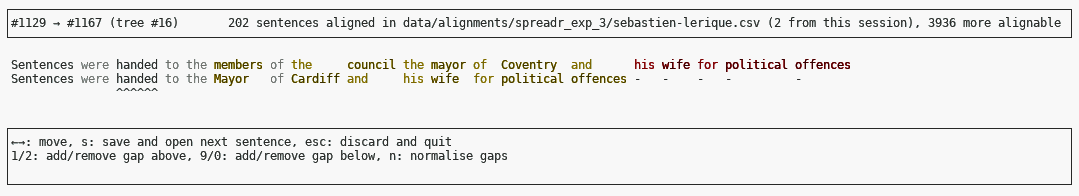
\includegraphics[width=\linewidth]{images/manual/gistr-goldcli-before.png}
  }

  \subfloat[After manual alignment]{
    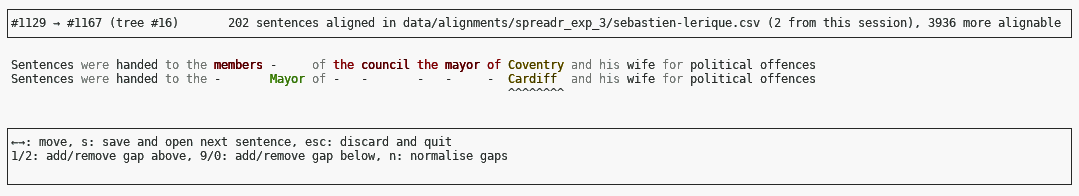
\includegraphics[width=\linewidth]{images/manual/gistr-goldcli-after.png}
  }
  \caption[Console interface for manual transformation alignment]{
  \textbf{Console interface for manual transformation alignment.}
  The user moves their cursor (underline below "handed" and "Cardiff") along the word sequences to insert or remove gaps and align the two utterances by hand.
  }
  \label{fig:gistr-goldcli}
\end{figure*}

Finally, we manually evaluated the overall quality of these parameters
by hand-coding the number of errors in a random set of 100 non-trivial
alignments generated by the parameters. Errors were counted as the
number of words whose alignment would have to be changed in order to
obtain a perfect alignment. Of those 100 alignments, 79 were perfect, 12
had 1 error, 4 had 2 errors, and the remaining 5 had between 3 and 6
errors. Counting 1 error as acceptable, this method yields a successful
alignment in 91\% percent of the cases. To make sure this is also the
case for deep alignments, we hand-coded errors in 100 random alignments
for which the algorithm had explored exchanges (though not all of them
are deep alignments, as it may be that the shallow alignment was the
best). An error was counted for each exchange that was missing,
mistaken, or should not have been present at all. Of the 100 alignments,
81 had no errors, 17 had 1, and 2 had 2 errors. The parameters obtained
here were thus used for all further analyses. They are also the ones
used in the example alignments discussed in the previous sections.

\subsection{Transformation model}\label{transformation-model}

The alignment procedure we just presented provides a list of deep
alignment trees for each transformation in the data set. At this point
we have showed that such deep alignments reliably encode the details of
a transformation broken down into smaller operations, thus completing
the first step of our modelling approach. We now proceed to the next
step: first, create an accurate visualisation of the details of
transformations captured by the alignments, then derive a transformation
model based on that visualisation. The step after that will then refine
the model and quantify the behaviours we can measure with it.

\subsubsection{Consensus filiations}\label{consensus-filiations}

The first step to visualise the process encoded by alignments is to
reduce the possibly multiple deep alignments encoding a transformation
into a single version, which we call the consensus alignment. Indeed for
a given transformation \(u \rightarrow u'\), a word in \(u\) could for
instance be assigned to different words in \(u'\) for different choices
of deep alignments. Other cases are possible, as \(w\) could be deleted
in one deep alignment and not in others, and so on and so forth. A
method to resolve conflicts across multiple deep alignments is therefore
required.

We adopt the following procedure to construct the consensus alignment
from the list of deep alignment trees of a transformation
\(u \rightarrow u'\). First, flatten each deep alignment tree into a
list. Recall that in a tree of deep alignments, a path from the root to
a leaf uniquely corresponds to one of the deep alignments encoded in the
tree: each tree encodes as many deep alignments as it has leaves. This
step thus takes each tree, and turns it into the list of deep alignments
that it encodes. Then, concatenate all the lists together. We are thus
left with a list of uniquely defined deep alignments for the
transformation. For instance, if we had \(n\) deep alignment trees with
\(m_1\), \ldots{}, \(m_n\) leaves in each tree, we now have a list of
\(m_1 + ... + m_n\) uniquely defined deep alignments.

Given this list of deep alignments, we then examine which operations are
present in the majority of the deep alignments. More precisely, for a
given word \(w\) in \(u\), determine if it is conserved either exactly
or through replacement in at least half of all the deep alignments. if
it is, then select the child word in \(u'\) which appears in most deep
alignments (i.e.~the majority child); if \(w\) is not conserved in at
least half of the deep alignments, then consider it deleted. Any word in
\(u'\) that has no assigned parent word is then considered an insertion.

A few details are worth mentioning here. First, a word that is stable in
exactly half the deep alignments and deleted in the other half is still
considered stable, such that the procedure sometimes maintains one or
two more stable words than the deep alignments it synthesises. Such
conflicts are inherent to any consensus method, and the alternative in
this case would be to consider the word unstable, adding deletions and
insertions instead of stabilities to the consensus alignment; we choose
to favour stabilities so as not to inflate operations artificially.
Second, an analogous conflict can arise when a stable word has two
equally probable candidate children, or conversely a given child word
has two equally probable parent words. In those cases we decide in
favour of the word closest to the end of the utterance, and the
procedure is consistent in both directions: the consensus alignment for
\(u \rightarrow u'\) is the same as for \(u' \rightarrow u\). Finally, a
small number of cases create new single-word exchanges, as two words are
assigned not the same child but different children at exchanged
positions; manual inspection of these cases showed that such exchanges
are consistent with the transformation they represent. In practice, only
53 of the 3461 transformations in Experiment 3 have more than one deep
alignment, 46 of which have 2 (the other seven having 3 to 6 deep
alignments), such that any change here has virtually no impact on the
results.

Now, consider for instance a simple branch
\(u \rightarrow u' \rightarrow u''\). A word \(w'\) in the middle
utterance \(u'\) is now uniquely identified (by the consensus alignment)
either as an insertion, or as the conservation or replacement of a
parent word \(w \in u\) (with or without movement due to an exchange).
Continuing down the branch, \(w'\) can also be linked to its child
\(w''\) (if it was not deleted), thus creating a lineage for this
specific word along the branch. Constructing consensus alignments for
each transformation thus allows us to follow the ancestry and descent of
individual words through parent and child transformations in a branch.

\subsubsection{Branch and utterance
dimensions}\label{branch-and-utterance-dimensions}

\Cref{fig:gistr-lineage-tree} represents the lineages produced by this
procedure on the branches of an example tree taken from Experiment 3,
whose root is the following utterance:\footnote{This is tree \#4, which
  is also shown in \cref{fig:gistr-trees}. The transition from depth 1
  to depth 2 in branch \#49 of the figure also corresponds to the
  transformation of utterance \ref{ut:49} to utterance \ref{ut:120}
  discussed when introducing deep alignments.}

\begin{nquote} % <!-- #4 -->
  « At Dover, the finale of the bailiffs' convention. Their duties, said a speaker, are "delicate, dangerous, and insufficiently compensated." »
\end{nquote}

\begin{figure*}[!h]
  \centering
  \includegraphics[width=\linewidth]{images/computed/exp_3/lineage-tree-4.png}
  \caption[Example lineages for all the branches of tree \#4 from Experiment 3]{
  \textbf{Example lineages for all the branches of tree \#4 from Experiment 3.}
  Each subplot corresponds to a different branch.
  The horizontal axis is the depth in the branch, and the vertical axis is the index of each word in its utterance.
  A grey line represents a word lineage along the branch, and the darkness of the line corresponds to the length of the path between the word's first appearance (or the branch start) and its disappearance (or the branch end);
  darker lines thus represent words that last longer across transformations (since branches eventually stop, however, our view of the process is truncated and the darkness is less reliable for words that appear towards the end of a branch).
  At each depth, the darker background band indicates what the subject sees, and the lighter band indicates the transformation that the subject made.
  Inside lighter bands:
  red dots are word deletions, green dots are word insertions, blue dots are word replacements, and exchanges can be seen when bundles of lines cross each other.
  Dots inside each light band are spread out on the horizontal axis so as make them easier to distinguish visually, but the horizontal position of a dot inside its band has no further meaning.
  }
  \label{fig:gistr-lineage-tree}
\end{figure*}

At first glance the plots reflect the rapid shortening of utterances,
and the fact that transformations are less important on shorter
utterances deeper in the branches. The figure also indicates that word
replacements, studied in the previous chapter with data from blogspace,
are quite speckled: they are less frequent than deletions and
insertions, and affect smaller portions of the utterances when they
appear. As replacements were the only process that could be extracted
from the blogspace data set, suspecting this caveat was one of the
motivations for our current experimental approach.

The plots also show noticeable regularities in the way transformations
vary. To discuss these we distinguish between the two axes of
\cref{fig:gistr-lineage-tree} as two scales of the representation, each
of which corresponds to a different set of events. First the horizontal
axis: an event at this level is the bulk transformation or conservation
of an utterance by a subject, without going into the detail of the way
an utterance changes. This yields a series of conservation and
transformation events, one at each depth in the branch. Call this the
branch dimension, pictured in \cref{fig:gistr-dimensions-branch}. A
salient feature on this dimension is the apparent burstiness of
transformations. Since successive subjects perform transformations
independently, confirming this trend would indicate a behaviour in
utterance evolution reminiscent of punctuated equilibria: a
transformation occurring after a period of stability would result in a
new utterance that is more likely to be transformed again. We quantify
this trend further down.

Second, the vertical axis which delves into the detail of a
transformation represented as a set of word insertions, deletions,
conservations and replacements with or without exchange. Call this the
utterance dimension. An important feature of this representation of
transformations is its uniqueness. Indeed, at the mathematical level a
consensus alignment encodes a transformation as a pair of word sequences
with gaps (and possible sub-alignments of exchanged parts), an encoding
that is not unique. Insertions and deletions that happen together can be
reordered (putting insertions before their neighbouring deletions
instead of the other way around, or alternating an insertion with a
deletion). The exchange of two parts around a stable chunk can also be
re-encoded by inverting the roles of stable and exchanged chunks, all
without changing the transformation represented by the encoding. By
compressing the gaps in this encoding, the utterance dimension merges
these equivalent versions together and produces a unique diagram
representing the transformation. We picture this correspondence between
the transformation diagram in the utterance dimension and the compressed
form of consensus alignments in \cref{fig:gistr-dimensions-utterance}.

\begin{figure*}[!h]
  \centering
  \subfloat[\textbf{Branch dimension.}
  This level looks at whether or not an utterance is transformed, without going into the detail of changes (hence the greyed out dots and lines).
  Similar to Fig.~\ref{fig:gistr-lineage-tree}, light grey bands are what subjects see, and the bands between those represent what the subjects do with what they read.
  An orange band indicates that an utterance was transformed, that is a T event, and a dark grey band indicates that an utterance was perfectly conserved, that is a C event.
  The corresponding ordered series of events is shown underneath the axis' arrow.]{
    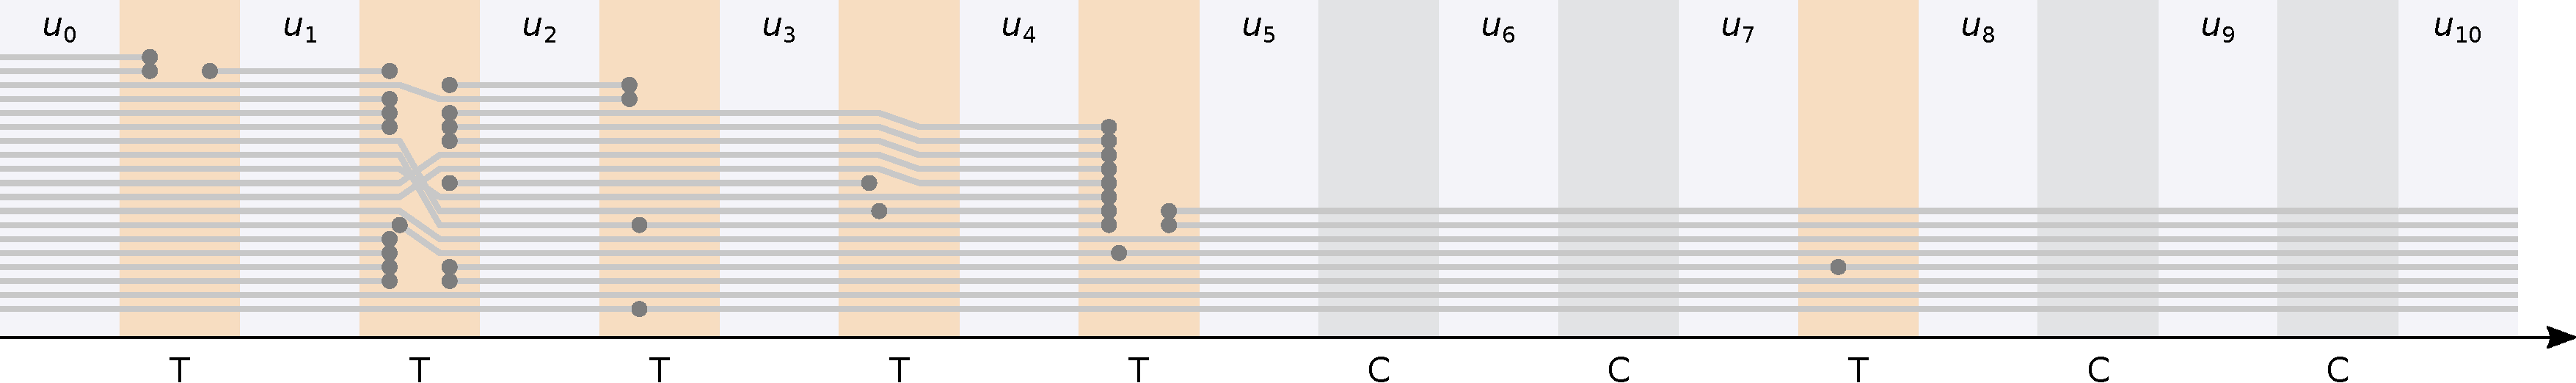
\includegraphics[width=\linewidth]{images/manual/gistr-dimensions-branch.pdf}
    \label{fig:gistr-dimensions-branch}
  }

  \subfloat[\textbf{Utterance dimension.}
  This level looks at the detail of a transformation, and represents it with a diagram that compresses the pair of sequences produced by aligning parent and child utterances.
  This diagram uniquely represents the transformation, and merges any variations in encoding that can exist in pairs of sequences with gaps.
  The top level of the figure shows how the canonical representation comes from the lineage plots.
  The bottom level shows two equivalent encodings of the same transformation (as would be produced by the alignment tool), which compress to the same canonical representation.]{
    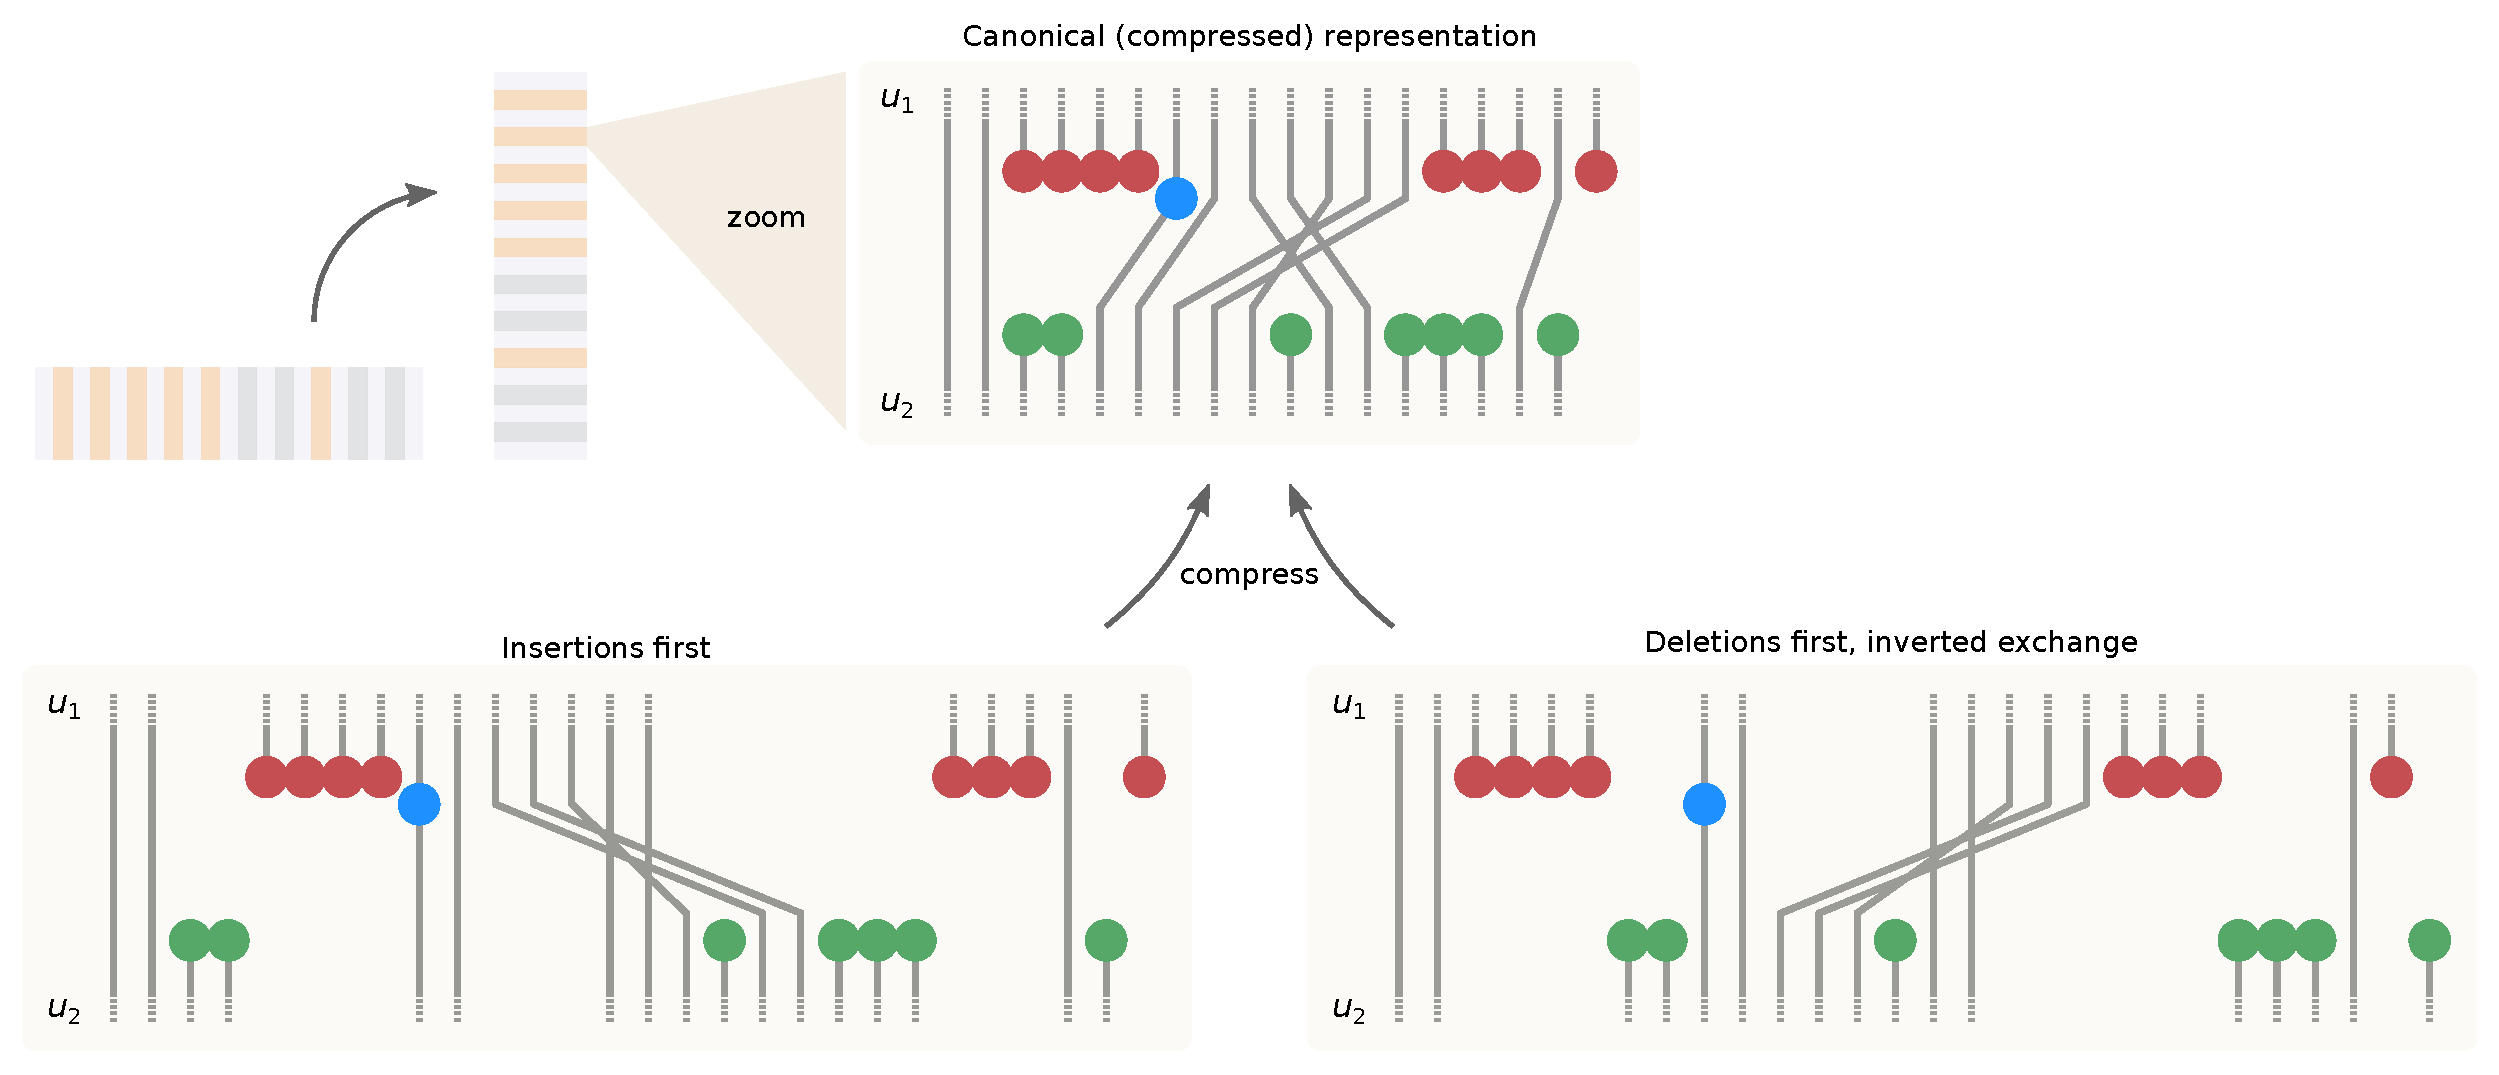
\includegraphics[width=\linewidth]{images/manual/gistr-dimensions-utterance.pdf}
    \label{fig:gistr-dimensions-utterance}
  }

  \subfloat[\textbf{Parent and child arrays of operations.}
  The canonical representation is further simplified by discarding the change in position encoded by word exchanges, and only keeping the information on whether a word is conserved or replaced.
  The procedure results in two arrays of word operations:
  a parent array made of conservations (C), replacements (R) and deletions (D), and a child array made of conservations, replacements and insertions (I).
  Conservations and replacements in the parent array, if not involved in exchanges, are linked to their corresponding operation in the child array, such that we can compute the distance between a block of insertions in the child and a block of deletions in the parent (except when exchanges separated the blocks).]{
    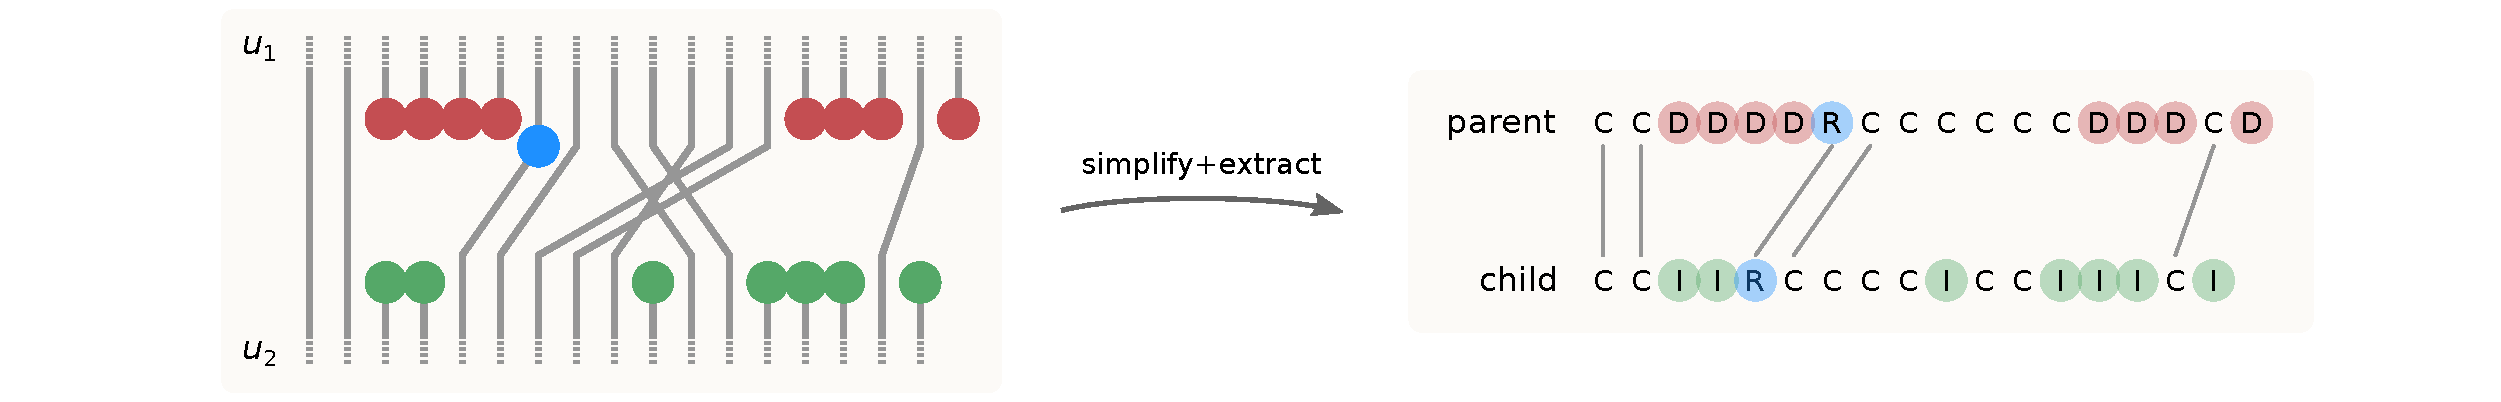
\includegraphics[width=\linewidth]{images/manual/gistr-utterance-arrays.pdf}
    \label{fig:gistr-utterance-arrays}
  }
  \caption[Analysis dimensions]{
  \textbf{Analysis dimensions.}
  Transformations are analysed along two dimensions.
  The branch dimension only looks at whether utterances are transformed or not, thus sees a series of T (transformed) and C (conserved) events.
  The utterance level looks at the detail of the transformations, and after simplification represents them with two arrays of operations, one for the parent utterance (made of C, R and D operations) and one for the child utterance (made of C, R and I operations).
  This example is built on branch \#49 from Fig.~\ref{fig:gistr-lineage-tree}.
  }
  \label{fig:gistr-dimensions}
\end{figure*}

This subtlety in the encoding of transformations is not a coincidence.
It relates to the fact that, in spite of the one-dimensional nature of
text written on a line, utterance transformation is a multi-level
process that can operate on whole groups of words at a time (for
instance when insertions and deletions happen together) and does not
necessarily reduce to a sequential series of events. Manually inspecting
the branches' transformations on the utterance dimension indicated
several trends to that effect, several of which are visible in
\cref{fig:gistr-lineage-tree}:

\begin{itemize}
\item
  Deletions, exchanges, and insertions seem bursty, that is they appear
  in large chunks (a behaviour that replacements do not seem to have).
  The bursts also seem longer if the utterance they appear in is longer.
\item
  Insertions seem to rarely occur without deletions. When they appear
  with deletions, the two tend to be close to each other and of similar
  magnitude.
\item
  All operations are less frequent at the very beginning of utterances.
\end{itemize}

As we just noted, burstiness at the word level is no surprise: words are
not processed independently and transforming parts of an utterance is
likely to depend on syntactic and semantic boundaries. However, the
behaviour of the bursts imposes constraints on the kind of model that
can account for the transformation process. In particular, the fact that
insertions and deletions seem to be of similar magnitude when close to
each other is not easy to account for. For instance, when creating an
insertion, a generative model must be aware of any deletions that have
already been created in the vicinity, and take their size into account.
Such a generative model would need to involve memory and attention span
mechanisms that allow bursts to relate to their neighbouring operations
(both preceding and following). Similarly, accounting for exchanges with
a generative model also requires at least a memory component that is
capable of recalling the postponed part of an exchange. Such mechanisms
are beyond the score of this chapter, and we therefore focus on
developing a descriptive---rather than generative---model. While it will
not allow for a reconstruction of the transformation process, this
approach will provide a synthetic understanding of the transformation
behaviour without needing to rely on cognitive mechanisms. By
abstracting out the basic building blocks of transformations, we will
then be able to gradually increase the level of detail with which we
understand the regularities of their interactions.

\subsubsection{Descriptive transformation
model}\label{descriptive-transformation-model}

Our model relies on a simplification of the transformation diagrams in
the utterance dimension of lineage plots, which we take to be the
canonical representation of a transformation. In order to keep the model
palatable, we first set aside part of the information provided by
exchanges. Indeed, the natural way of analysing an exchange in a
transformation diagram is to see it as a permutation of a sub-sequence
of words in the utterance, with possible replacements, insertions and
deletions added in-between. Analysing the regularities of such a process
is matter for a model in itself, and we chose to leave this aspect of
transformations for further research. We instead focus on insertions,
deletions and replacements only. When words are exchanged we consider
only whether they are replaced or conserved, and do not look at their
change of position. Note that while this excludes any shifts in position
from our model, the approach still benefits from having detected
exchanges earlier in the procedure: it guarantees that the remaining
insertions and deletions correspond to actual appearances and
disappearances, not undetected exchanges.

From a given transformation diagram we then extract two arrays of
word-level operations,\footnote{We use the phrase \enquote{array of
  operations}, and not \enquote{series of events}, to emphasise that
  these operations exist on the one-dimensional utterance axis, but do
  not necessarily come from a sequential generation process. The two
  terms refer to the same mathematical object, and simply change the
  interpretation of the index: for a series of events the index
  represents time, for an array of operations it does not.} one for the
parent utterance and one for the child utterance. Parent and child
arrays both may contain conservation and replacement operations, and
parent arrays may contain deletion operations while child arrays may
contain insertion operations. The transformation diagram further
provides us with the correspondence of conservation and replacement
operations between the two arrays (except for operations that were
involved in an exchange, for which we lose position information), such
that we can measure the distance between two blocks of insertions and
deletions (except if the two blocks are separated by operations involved
in an exchange).

\Cref{fig:gistr-utterance-arrays} illustrates this simplification of
transformations, which we use as our model for the process: it
represents a transformation as two arrays of word-level operations, one
for the parent utterance made of word conservations, replacements, and
deletions, and one for the child utterance made of word conservations,
replacements, and insertions. Some operations happen on several
contiguous words at a time, and we call these \emph{chunk-level
operations}. Conversely, when referring to operations defined as single
word insertions, deletions, replacements or conservations, we will use
the phrase \emph{word-level operation}, or simply \emph{operation} when
the context is clear. Contiguous word-level operations, then, form a
single chunk-level operation.

Note that a word-level conservation or replacement in one array can
additionally, but not necessarily, be paired with another word-level
conservation or replacement in the other array. Thus, when chunk-level
insertions and deletions are separated by paired conservations or
replacements, we define the distance between the two chunk-level
operations as the number of conservations or replacements separating the
two. For instance, a chunk-level insertion can appear two words after a
chunk-level deletion, and this information will be useful when comparing
the sizes of chunk-level insertions and deletions in a given
transformation. When unpaired conservations or replacements separate
chunk-level insertions and deletions, however, this distance will remain
undefined.

\subsection{Model refinement}\label{sec:gistr-results-inner}

Having defined our model for transformations, we now delve into the
detailed behaviour that it captures. We do so in three stages. First, we
quantify the extent to which transformations are bursty, both in the
branch dimension and in the detailed transformation model (utterance
dimension). In doing so we establish the prevalence of chunk-level
operations in the transformation model. We then characterise the number
of word-level and chunk-level operations that occur in utterances,
linking their magnitude and probability to the length of the parent
utterance and the position at which they occur. Finally, we examine the
dependencies between each operation type, and highlight a close
relationship between insertions and deletions.

\subsubsection{Bursty behaviours}\label{bursty-behaviours}

We begin by measuring the extent to which each dimension features bursty
behaviour. Following \textcite{jo_circadian_2012}, who rely on
\textcite{goh_burstiness_2008}, we measure the burstiness of a series of
events through the parameter \(B\) defined as

\[B = \frac{\sigma_{intervals} - \mu_{intervals}}{\sigma_{intervals} + \mu_{intervals}}\]

where \(\sigma_{intervals}\) and \(\mu_{intervals}\) are respectively
the standard deviation and mean of the distribution of inter-event times
in the series of events. The same computation applies to arrays of
operations (the two have the same mathematical description). \(B\) has
values between -1 and 1; \(B = -1\) corresponds to a perfectly regular
process (\(\sigma_{intervals} = 0\), and \(\mu_{intervals} > 0\) is the
constant period of events), \(B = 0\) indicates a burstiness similar to
that of a Poisson process, where the occurrence of a new event does not
depend on the presence of previous events (and
\(\sigma_{intervals} = \mu_{intervals}\)), and \(B = 1\) corresponds to
an asymptotically perfectly bursty process (it is the limit
\(\sfrac{\mu_{intervals}}{\sigma_{intervals}} \rightarrow 0\)).
Intuitively, a process with average inter-event time shorter than its
standard deviation will often have events close to each other with a few
long intervals without events, and a process with an average inter-event
time longer than its standard deviation will have events more evenly
spaced relative to their mean spacing.

Note that this measure can be applied to any series of events, and we
therefore use it in both the utterance and the branch dimensions. In the
utterance dimension, it tells us the extent to which the changes that a
subject makes in an utterance tend to occur in contiguous chunks. We
will see that this chunkiness is very strong, so much that we will start
examining insertions and deletions and the level of chunks. In the
branch dimension, the measure tells us how bursty the evolution along a
branch is. A bursty evolution would indicate a punctuated equilibria
behaviour, with long periods of stability interrupted by sudden bursts
of transformations. A non-bursty behaviour would indicate that a
subject's transformations do not influence the following subject so
much.

Let us start with the utterance dimension. In the parent array, we note
the series of deletion events \(\mathcal{D}\) and the series of
replacements \(\mathcal{R}_p\). In the child array, we note the series
of insertion events \(\mathcal{I}\) and the series of replacements
\(\mathcal{R}_c\). A conserved word is considered an absence of event.
Note that because of inserted and deleted words, replacements may not
appear with the same distributions in the parent and child arrays. As a
consequence, \(\mathcal{R}_p\) and \(\mathcal{R}_c\) may not have the
same distribution of inter-event times. The burstiness measures for each
of these series are shown in
\cref{fig:gistr-utterance-burstiness-words}, along with the burstiness
of the series made of all parent or child events without distinguishing
their type. The plots show that deletions and insertions are both
bursty, while replacements are undistinguishable from a non-bursty
process such as a Poisson process. When all event types are joined
together, the process is also bursty, albeit slightly less.

Given the strength of this behaviour for deletions and insertions, we
further look at these series by collapsing each contiguous set of
deleted or inserted words into a single event. This leads to a series of
chunk-level deletions and insertions separated by word-level
replacements and conservations (non-events). For inter-event times, this
corresponds to removing the null values in the previous distributions of
inter-event times (which separated words in the same chunk-level
operation); computing the burstiness of the chunk-level process is
therefore straightforward. The values plotted in
\cref{fig:gistr-utterance-burstiness-chunks} show that none of the
chunk-level processes are bursty; rather, they are slightly more regular
than a Poisson process would be.

\begin{figure*}[!ht]
  \centering
  \subfloat[Burstiness of word-level operations]{
    \includegraphics[width=.55\linewidth]{images/computed/exp_3/burstiness-words.png}
    \label{fig:gistr-utterance-burstiness-words}
  }
  ~
  \subfloat[Burstiness of chunk-level operations]{
    \includegraphics[width=.40\linewidth]{images/computed/exp_3/burstiness-chunks.png}
    \label{fig:gistr-utterance-burstiness-chunks}
  }
  \caption[Burstiness of operations in the utterance dimension]{
  \textbf{Burstiness of operations in the utterance dimension.}
  The left pane shows the burstiness of each type of word-level operation in parent and child arrays, as well as the burstiness of the series made of all operations joined regardless of their type.
  The right pane shows the burstiness for deletions, insertions, and joined events, where contiguous sets of operations are collapsed into single events.
  This corresponds to the burstiness of chunk-level deletions, insertions, and joined events.
  Grey lines are the 95\% confidence intervals based on Student's $t$-distribution, considering each tree as an independent burstiness measure.
  }
  \label{fig:gistr-utterance-burstiness}
\end{figure*}

Although this behaviour is consistent with our intuition of the way an
utterance is reformulated, there is a question as to whether the
alignment procedure does not favour burstiness. Indeed, the scores of
operations are parametrised in such a way that insertion and deletion
gaps are assigned different costs for initial opening and extension.
However, while this parametrisation makes it possible for burstiness to
be more easily identified, it does not make it a necessity: setting the
gap opening cost to the same value as the gap extension cost would make
the alignment tool neutral with respect to burstiness (setting it lower
would be biased against burstiness, and the alignment algorithm would
favour word mismatches over gaps to encode differences). In our case,
the parameters we trained set the gap opening cost to a much higher
value than the extension cost (.29 vs. .12 in absolute values), such
that the alignment tool does find bursty insertions and deletions more
easily. However, these parameters are learned from hand-coded alignments
and their output has been validated on test samples: any bursty
insertions or deletions detected by the alignments is therefore the
product of the data itself, and not an artefact.

Let us now step back and look at the evolution along the branches, that
is, the branch dimension. We ask whether the fact that an utterance is
transformed has an effect on the subsequent transformations by other
subjects. Here the situation involves only one event type: the
transformation of an utterance is an event, and the conservation of an
utterance is the absence of an event. Note that our data in this
dimension is truncated due to branches not being infinite. When the last
subject in a branch does not transform the utterance they reproduce, we
do not observe the actual duration of that stability: had the branch
continued, the stability could have been interrupted immediately, or
could have lasted for many more reproductions of the utterance.
Including these truncated intervals in the distribution of inter-event
times artificially inflates the burstiness (because it adds
underestimated intervals to the distribution), but removing them biases
our sample towards inter-event times for longer utterances (earlier in
the branch), which could also inflate burstiness. We thus present
measures for both distributions, with and without the truncated
intervals.

Burstiness in the branch dimension with truncated intervals is
\(B_{branch,all} = 0.252 \pm 0.029\), and burstiness without the
truncated intervals is \(B_{branch,observed} = 0.304 \pm 0.031\) (both
error estimates correspond to the 95\% confidence interval based on
Student's \(t\)-distribution, considering each tree as an independent
burstiness measure). Both measures show that the transformation process
in the branch dimension is significantly bursty. This is consistent with
our intuition that when a transformation appears after a period of
stability, it is likely to trigger other transformations following it
until a new stable (often much shorter) utterance is reached.

\bigskip
Overall, it appears that insertions and deletions inside an utterance
tend to cluster into chunks, which is not a surprise as sentence
processing does not happen at the word-level only. Still, this makes the
chunk-level of analysis relevant for what follows. Replacements,
conversely, do not appear in chunks, and chunk-level operations
themselves also do not cluster into higher-kinded chunks. Interestingly,
the evolution along branches is also bursty, although this is due to an
entirely different process: the measure suggests that when one subject
transforms a previously stable utterance, the new production is itself
more susceptible to further transformations that could be regularising
the changes introduced by the first subject.

\subsubsection{Position and utterance
length}\label{position-and-utterance-length}

The general trends presented in \cref{sec:gistr-results-general}
indicated that utterance length has a strong effect on the probability
and magnitude of transformations. The transformation models now lets us
explore in detail the way word-level and chunk-level operations depend
on the size of an utterance, on one side, and on the position at which
they occur, on the other.

We begin by looking at the probability of each operation as a function
of utterance length. \Cref{fig:gistr-ops-prob} plots the logistic
regression of the presence or absence of deletions, insertions, and
replacements as a function of the number of words in the parent
utterance. The length of the parent utterance has a significant effect
on all three operations, with deletions being the quickest to increase
in probability, followed by replacements then insertions: the threshold
for having deletions over half the time is 19 words, 22.6 for
replacements, and 28.1 words for insertions; the slopes of the
regressions are also ordered this way. In other words, a longer
utterance will have a higher risk for all operations, and the increase
is strongest for deletions, then for replacements, then for insertions.

\Cref{fig:gistr-ops-count} further shows the number of operations as a
function of parent utterance length, either counting one for each
word-level operation or counting one for each chunk-level operation. The
number of word-level and chunk-level operations increase close to
linearly as a function of parent length. Deletions have by far the
strongest link to parent length, both at the word and chunk levels,
followed by insertions then replacements. Note that the replacement
counts barely change between word and chunk level since this operation
is not bursty: it affects mostly isolated words instead of contiguous
sets of words. In short, a longer utterance has a higher probability of
suffering any type of operation, with on average over a quarter of the
words deleted, the equivalent of a fourteenth of the original utterance
in new words, and about a twentieth of the words replaced.

\begin{figure}[!ht]
  \centering
  \subfloat[\textbf{Probability of word operations w.r.t. parent length.}
  Computed as the log-odds logistic regression of the presence or absence of a given operation in the transformation of $u_p$ (parent) into $u_c$ (child), versus the number of words in $u_p$.
  Colours correspond to the colour-coding used in Fig.~\ref{fig:gistr-lineage-tree}.
  Light shades are 95\% regression confidence intervals.]{
    \includegraphics[width=\linewidth]{images/computed/exp_3/p-ops_parent-length_logistic.png}
    \label{fig:gistr-ops-prob}
  }

  \subfloat[\textbf{Number of word-level and chunk-level operations w.r.t. parent length.}
  Parent lengths are binned into 5 quantile-based bins.
  The word-level counts the number of individual words affected by an operation (deletion, insertion, replacement).
  The chunk-level counts the number of contiguous sets of words affected by an operation.
  Light shades are 95\% regression confidence intervals, and vertical bars are 95\% confidence intervals for the value of a bin (Student $t$-based, here counting each operation as an independent measure).
  % \todo{FIXME: vertical bars should count each transformation as independent}
  ]{
    \includegraphics[width=\linewidth]{images/computed/exp_3/chunk-size_parent-length.png}
    \label{fig:gistr-ops-count}
  }
  \caption[Probability and number of word-level or chunk-level operations]{
  \textbf{Probability and number of word-level or chunk-level operations.}
  }
  \label{fig:gistr-ops-counts}
\end{figure}

Manual exploration of the lineage plots also indicated that operations
are not positioned evenly in the utterances. To quantify this behaviour
we apply the susceptibility measure developed in the previous chapter to
positions in an utterance. For words at position \(x \in [0, 1]\)
relative to their utterance's length (\(x = 0\) for words at the
beginning, \(x = 1\) for words at the end), the susceptibility
\(\sigma_O(x)\) to an operation \(O \in \{D, I, R\}\) is defined as the
ratio of \(s_O(x)\), the number of times words at relative position
\(x\) are the target of operation \(O\), to \(s_O^0(x)\), the number of
times those words would be the target of operation \(O\) if the choice
of words were random:\footnote{Since operations in a given
  transformation are not independent, we scale both \(s_O(x)\) and
  \(s_O^0(x)\) such that each transformation has a maximum contribution
  of 1 to the total counts. This procedure is similar to the
  susceptibility scaling approach we followed in the previous chapter.}

\[\sigma_O(x) = \frac{s_O(x)}{s_O^0(x)}\]

\Cref{fig:gistr-susc-ops} plots \(\sigma_D\), \(\sigma_I\) and
\(\sigma_R\) (for replacements on the parent side) both overall and for
binned parent lengths. The leftmost plots show that deletions and
insertions are half as likely to appear at the very beginning of an
utterance as they would at random, and more likely than random in the
second half of an utterance. This is consistent with the well-known
primacy effect in recall of word lists. In this case, subjects transform
the beginning of an utterance on average much less than the rest.
Replacements feature this primacy effect to a lesser extent, with the
addition of a slight recency effect: words at the end of an utterance
are slightly less replaced than non-extremity words. The plots at binned
parent lengths show little to no variation in these patterns: each
pattern is more or less marked depending on the parent sentence length
(especially for replacements, which seem more uniform for short
utterances), but the general behaviour is the same for different parent
lengths.

\begin{figure}[!ht]
  \centering
  \subfloat[Deletions]{
    \includegraphics[width=\linewidth]{images/computed/exp_3/susceptibility-del_position_parent-length.png}
    \label{fig:gistr-susc-del}
  }

  \subfloat[Insertions]{
    \includegraphics[width=\linewidth]{images/computed/exp_3/susceptibility-ins_position_parent-length.png}
    \label{fig:gistr-susc-ins}
  }

  \subfloat[Replacements]{
    \includegraphics[width=\linewidth]{images/computed/exp_3/susceptibility-rpl_parent_position_parent-length.png}
    \label{fig:gistr-susc-rpl}
  }
  \caption[Susceptibility for word operations as a function of relative position in the utterance]{
  \textbf{Susceptibility for word operations as a function of relative position in the utterance.}
  The leftmost plot of each sub-figure (blue background) shows $\sigma$ computed over all transformations.
  The plots with the white backgrounds show $\sigma$ computed over transformations with binned parent utterance lengths, indicated in the plot titles.
  Parent length bins are quantile-based, that is computed to have the same number of utterances in each bin (the bins are identical to Fig.~\ref{fig:gistr-ops-count}).
  Light shades are the 95\% confidence intervals computed following the \textcite{goodman_simultaneous_1965} method for multinomial proportions, considering each transformation as an independent measure.
  }
  \label{fig:gistr-susc-ops}
\end{figure}

Finally, we examine the dependence of chunk-level operation size on its
position in an utterance. The manual exploration of lineage plots did
not hint to any effect at this level, but the question now appears
legitimate: since subjects delete words on average more often towards
the end of an utterance, it is possible that those deletions are also
longer if they correspond to larger memory loss.
\Cref{fig:gistr-chunk-size} shows the dependence of chunk-level
operation size on position in the utterance, for deletions, insertions
and replacements, both overall and for binned parent length. Deletions
exhibit a slight effect of position on chunk-level operation size, which
is significant for parent lengths between 11 and 15 words.\footnote{The
  plots also indicate that the overall chunk-level operation size
  increases with parent length, a slight effect which was confirmed for
  deletions and insertions with dedicated regressions, but which we do
  not discuss further given its mildness (slopes respectively .030 and
  .013, both significative with \(p < .001\)).} That is, for those
lengths, deletions towards the end of the utterance are significantly
larger than deletions at the beginning (4.1 words versus 1.7 words on
average), in addition to being more frequent (see the susceptibility
plots above). The trend is present for deletions at all lengths, though
most of the time not significative. Other operations do not seem to
exhibit this behaviour (the variations for insertions are not
significative).

\begin{figure}[!ht]
  \centering
  \includegraphics[width=\linewidth]{images/computed/exp_3/chunk-size_position_parent-length.png}
  \caption[Chunk-level operation size w.r.t. parent length and position in utterance]{
  \textbf{Chunk-level operation size w.r.t. parent length and position in utterance.}
  The leftmost plot (blue background) shows the average chunk-level operation size w.r.t. parent length for all utterances.
  The plots on its right (white background) divide that data into binned parent lengths (bins identical to Figs.~\ref{fig:gistr-ops-count}--\ref{fig:gistr-susc-ops}).
  In each plot, the height of a line for a given relative position $x$ corresponds to the average size of the chunk-level operations in which words at position $x$ are found;
  for instance, a chunk-level deletion that spans the second half of an utterance will be spread over $x \in [.5, 1]$.
  Average sizes are weighted such that each utterance contributes 1 unit.
  Light shades are the 95\% confidence intervals (Student $t$-based, considering each transformation as an independent measure).
  }
  \label{fig:gistr-chunk-size}
\end{figure}

Overall, these measures show that deletions are more frequent than
insertions, which are more frequent than replacements. Operations happen
preferentially in the second half of utterances (except replacements
which favour all positions except extremities), and the number of
word-level and chunk-level operations are proportional to the parent
length. Chunk-level deletions are also larger in the second half of
utterances, compared to in the first half.

\subsubsection{Dependencies between
operations}\label{dependencies-between-operations}

Manual exploration of the lineage plots indicated that operations have
non-trivial dependencies between each other. The contingency table
combining the presence or absence of each operation gives an overview of
these dependencies:

\begin{center}
  \begin{tabular}{llrrrr}
    \toprule
     & & \multicolumn{4}{c}{\textbf{Deletion}} \\
    \cmidrule(l){3-6}
     & & \multicolumn{2}{c}{\emph{no}} & \multicolumn{2}{c}{\emph{yes}} \\
    \cmidrule(lr){3-4} \cmidrule(l){5-6}
    \multicolumn{2}{l}{\textbf{Replacement}} & \multicolumn{1}{c}{\emph{no}} & \multicolumn{1}{c}{\emph{yes}} & \multicolumn{1}{c}{\emph{no}} & \multicolumn{1}{c}{\emph{yes}} \\
    \midrule
    \multirow{2}{*}{\textbf{Insertion}} & \emph{no} & 1381 & 415 & 286 & 308 \\
     & \emph{yes} & 66 & 94 & 399 & 512 \\
    \bottomrule
  \end{tabular}
\end{center}

\begin{figure}[!ht]
  \centering
  \includegraphics[width=.6\linewidth]{images/computed/exp_3/contingencies_mosaic.png}
  \caption[Mosaic plot of the contingency table between deletions, insertions, and replacements]{
  \textbf{Mosaic plot of the contingency table between deletions, insertions, and replacements.}
  Red rectangles indicate deletions are present;
  green rectangles or green dots indicate insertions are present;
  darker colours indicate replacements are present.
  Each rectangle also indicates the number of transformations it represents (corresponding to the rectangle area).
  }
  \label{fig:gistr-contingencies}
\end{figure}

\Cref{fig:gistr-contingencies} illustrates this data with a mosaic plot,
rendering some of the trends more visible. One way to look at these
figures is by considering deletions first. Without deletions, insertions
are very unlikely (8.2\%), and replacements are also unlikely (though
less so: 26.0\%): the most likely event without deletion is by far a
transformation with no change at all (70.6\%). With deletions, all four
possibilities are of comparable probabilities: having both insertions
and replacements is the most likely case (34.0\%), followed by
insertions without replacements (26.5\%), then replacements without
insertions (20.5\%), then neither replacements nor insertions (19.0\%).
Overall, deletions can be seen as a gate for other transformations:
without them the most likely outcome is no change at all, with them all
situations have relatively similar probabilities. A second way to look
at the contingencies is to consider that insertions trigger deletions:
without insertions, deletions happen only 24.9\% of the time, whereas
with them deletions are extremely likely (85.1\%). Replacements are also
linked to insertions, either with or without deletions: the presence of
one always increases the probability of the other.

\begin{figure}[!ht]
  \centering
  \subfloat[Number of insertions conditioned on the presence of deletions.]{
    \includegraphics[width=.4\linewidth]{images/computed/exp_3/insertion-lv_del-presence.png}
    \label{fig:gistr-ins-lv}
  }
  ~
  \subfloat[Number of deletions conditioned on the presence of insertions.]{
    \includegraphics[width=.4\linewidth]{images/computed/exp_3/deletion-lv_ins-presence.png}
    \label{fig:gistr-del-lv}
  }
  \caption[Deletion and insertion counts conditioned on the presence of one another]{
  \textbf{Deletion and insertion counts conditioned on the presence of one another.}
  All distributions of operation counts are shown as letter-value plots \autocite{hofmann_letter-value_2011}.
  The left panel shows that utterances where a deletion is present also have many more insertions than if there were no deletions (the red distribution reaches much higher numbers of insertions than the grey distribution).
  Similarly in the right panel, deletions appear in greater numbers in utterances that have an insertion.
  (More technically, in a given plot the boundaries between boxes are placed at the $2^i$-th quantiles:
  the middle line is the median, and above and below it the biggest box stops at the first and third quartiles, such that it contains half the data points;
  the second biggest box stops at the first and seventh 8-quantiles, i.e. octiles, and so on and so forth.
  Diamonds are outliers that do not fit into the smallest box.)
  }
  \label{fig:gistr-insdel-lv}
\end{figure}

The process is joint of course, and separating it into different stages
would require more knowledge of the cognitive mechanisms that underlie
these transformations. In spite of this, the relationship between
insertions and deletions seems to be well constrained, a fact we see not
only in the probability of presence or absence, but also in the number
of operations inside a given transformation. The link between insertions
and deletions can be seen by plotting the distribution of the number of
insertions conditioned on the presence of deletions, and vice-versa.
Both plots are shown on \cref{fig:gistr-insdel-lv}: aside from being
less probable, insertions without deletions are also much smaller in
number compared to with deletions. A similar behaviour is observed in
the opposite case: deletions that happen in the presence of an insertion
are much greater in number than without insertions.

Deletions and insertions thus seem closely linked, as our intuition of
the process suggests: deletions could be the first manifestation of the
subject having forgotten something in the parent utterance, and their
presence then opens the door to further reformulations, possibly to make
up for the forgotten content.

This relates to the last observation produced by our manual exploration:
chunk-level insertions and deletions seem to occur in similar sizes when
close to one another. To quantify this observation we estimate a
correlation function between the sizes of chunk-level insertion and
deletion separated by fixed numbers of conserved or replaced words. More
precisely, for each chunk-level insertion in the data set we identify
the nearest chunk-level deletion either before or after it, separated by
words that are not involved in an exchange.\footnote{As alluded to when
  introducing the transformation model, when exchanges separate a
  chunk-level insertion from a chunk-level deletion there are several
  paths from one to the other, depending on when one traverses the
  exchange; different paths can have different final distances, none of
  which are more or less plausible than the others. The distance between
  a chunk-level insertion and a chunk-level deletion separated by an
  exchange is thus not clearly defined.} If a chunk-level insertion has
such a nearest neighbour (it may not if there were no deletions, or if
it occurred in the middle of exchanged words such as in
\cref{fig:gistr-utterance-arrays}), we note \(r\) the separation between
the two chunk-level operations. If chunk-level insertion and deletion
face each other, \(r = 0\); otherwise, \(r < 0\) if the deletion comes
before the insertion in the utterances, \(r > 0\) if the deletion comes
after, and \(|r|\) equals the number of conserved or replaced words
separating the two. For a given value of \(r\), we compute a robust
linear regression of chunk-level insertion size against chunk-level
deletion size for all insertion-deletion chunks separated by \(r\). We
then take the slope of that regression as an indicator of the
correspondence between the sizes of \(r\)-separated chunk-level
insertions and deletions.\footnote{The robust regression lets us
  minimise the impact of outliers in the distributions of chunk-level
  insertion sizes, which otherwise had a strong effect on more common
  correlation measures. The regression is computed using the Statsmodels
  statistics library for Python, which implements robust M-estimation
  using Huber's T norm \autocite{huber_robust_1981} with a default
  parameter of 1.345.}

\begin{figure}[!ht]
  \centering
  \includegraphics[width=\linewidth]{images/computed/exp_3/insdel_distance_size.png}
  \caption[Size correlation between nearest-neighbour chunk-level insertions and deletions at different distances]{
  \textbf{Size correlation between nearest-neighbour chunk-level insertions and deletions at different distances.}
  The bottom subplots show the robust regressions for couples of insertion-deletion chunks separated by a given value of $r$.
  The text at the top of each subplot indicates the number of insertion-deletion couples that the subplot represents.
  The top plot shows the values of the regression slopes aligned to the bottom subplots, with 95\% regression confidence intervals and star-coded significance levels (*** for $p < .001$, ** for $p < .01$, * for $p < .05$ and nothing otherwise).
  }
  \label{fig:gistr-insdel-correlations}
\end{figure}

\Cref{fig:gistr-insdel-correlations} shows the robust regressions and
the estimated correlation function for \(r \in \{ -5, ..., 5 \}\)
(outside of which there was always less than 10 insertion-deletion
couples). The plot shows three important points. First, the vast
majority of nearest neighbours insertion and deletion chunks face each
other (\(r = 0\)), and their sizes significantly correlate. Second, the
correlation initially decreases to become non-signifcant as \(|r|\)
increases. The third and most interesting point is that the correlation
function is skewed towards the left: it is significantly above zero for
\(r = -1\) but not for \(r = 1\), then also for \(r = -4, -5\) at higher
values than for \(r = 4\). Note however that the last three points
represent only 10 to 12 chunk-level insertion-deletion couples each and
are thus more susceptible to outliers (especially to deletion outliers,
i.e.~the x axis, which the M-estimation technique we used does not
counter). Overall, the correlation is positive for chunk-level
insertions and deletions facing each other, and also often for
chunk-level deletions preceding insertions by a few words.\footnote{The
  detail of these plots is sensitive to cropping in the data, and
  especially to constraints on the maximum chunk-level deletion size
  since it can remove x-axis outliers. The general trend we observe is
  always conserved however: deletions preceding insertions correlate
  more than deletions following insertions.} This trend is consistent
with the intuition we outlined above, according to which chunk-level
insertions could come as tentative replacements for the content that was
lost in the deletions that directly precede them.

\bigskip
The transformation model we introduced thus captures several important
behaviours in the way subjects change utterances. Looking at
transformations as made of word-level replacements, deletions and
insertions, we see that both insertions and deletions are bursty, and
that the presence and magnitude of an operation depends strongly on
utterance size and the position at which it appears in the utterance. We
further see that chunk-level insertions and deletions are closely
related: insertions behave as if they were gated by the presence of a
deletion, and their sizes tend to correlate to that of deletions
appearing at the same time or shortly before them.

\subsection{Lexical feature makeup}\label{lexical-feature-makeup}

We finally descend to the lower level of lexical word features to
characterise the words involved in insertions, deletions and
replacements. We thus extend the feature analysis of the previous
chapter to our current situation, and verify the consistency of the new
results with previous word susceptibility and feature variation
measures. Finally we extend the analysis to a point we could not reach
in the previous data set, by looking at the accumulation of
transformations along the branches and the evolution they cause in the
lexical makeup of utterances.

\subsubsection{Word features}\label{word-features}

For the sake of conciseness, we restrict features to the four lexical
variables that showed relevant effects in the previous chapter: word
frequency, age of acquisition, Free Association clustering and number of
letters, thus leaving aside number of synonyms and orthographic
neighbourhood density. Age of acquisition, clustering and (obviously)
number of letters are identical to the previous chapter. Word frequency
was previously computed from the complete set of online quotations;
however, since the present data set is much smaller we relied instead on
external word frequency ratings based on subtitles
\autocite{heuven_subtlex-uk:_2014}, a source which has repeatedly beaten
previous predictors of standard lexical decision times \autocite[see][
for more details]{heuven_subtlex-uk:_2014}. These frequencies are
provided on what the authors introduce as the Zipf scale, computed as
\(\log_{10}(\text{Frequency per billion words})\). The frequency values
thus use a different source than those of the previous chapter, but
their final computation only differs by an affine transformation.

The situation is otherwise parallel to that of the previous chapter, and
its procedure can be directly applied. We measure the susceptibility of
words to being the target of an operation (either by deletion or
replacement) in a similar manner to substitution susceptibility. We
additionally measure the susceptibility to being the new word of an
operation (either as replacing word or inserted word). For a given
grouping of words \(g\) (e.g.~grammatical category or feature value), we
compute its susceptibility \(\sigma_g^-\) to being a target and its
susceptibility \(\sigma_g^+\) to newly appearing as the ratio of the
number of times it is a target (\(s_g^-\)) or a new word (\(s_g^+\)) to
the number of times it would be if the process were a random sampling
from the available utterances (\(s_g^0\)):

\[\sigma_g^- = \frac{s_g^-}{s_g^0} \quad \text{and} \quad \sigma_g^+ = \frac{s_g^+}{s_g^0}\]

Together, these measures provide a more precise view of susceptibilities
than the one we had in the previous chapter: first, the measures
integrate insertions and deletions as well as replacements (more
generally, here we see all possible operations, when the previous
chapter had to be restricted to single-word substitutions); second, we
distinguish the susceptibility to appearing from the susceptibility to
disappearing, thus allowing us to compare the types of words that
disappear to the types of words that appear.

\begin{figure}[!ht]
  \centering
  \includegraphics[width=.75\linewidth]{images/computed/exp_3/pos-suscept-rplinsdel.png}
  \caption[POS susceptibility to targeting and to appearance]{
  \textbf{POS susceptibility to targeting and to appearance.}
  Targeting, that is on the parent side, can be either deletion or replacement;
  appearance, that is on the child side, can be either insertion or replacement.
  The top panel shows the proportions of POS categories observed in utterances overall ($s_{POS}^0$), in targeted words ($s_{POS}^-$) and in appearing words ($s_{POS}^+$).
  The bottom panel shows susceptibilities, that is the ratio of $s_{POS}^-$ and $s_{POS}^+$ to $s_{POS}^0$.
  95\% asymptotic confidence intervals are shown in grey (Goodman-based multinomial proportions, considering each transformation as an independent measure).
  POS tags are from the Universal Dependencies tag set.
  }
  \label{fig:gistr-suscept-pos}
\end{figure}

In order to render the results more comparable to the previous chapter,
in this subsection we also filter out stopwords in all the utterances.
\Cref{fig:gistr-suscept-pos} shows the behaviour for grammatical
categories, plotting \emph{Part-of-Speech} (POS) susceptibilities for
being the target or the new word of an operation. The two measures are
very close to each other, and similarly to the online case there is
little to no effect of the main categories on susceptibility: adjectives
are involved at random, nouns appear slightly less than at random, and
verbs slightly more. Verbs, nouns and proper nouns are all irrelevant
for targeting, but adverbs are targeted very slightly above random. The
other categories (adpositions, numerals and particles) total negligible
amounts because they are affected by the stopword filter. Overall, the
behaviour for targeting is consistent with what we observed in blogspace
(the only difference being the trend for adverbs, which are also less
present overall in this data set), and the behaviour for appearances
indicates a slight bias in favour of verbs and against nouns (note that
appearance susceptibilities were not analysed in the blogspace data set,
so we have no point of comparison).

\begin{figure}[!ht]
  \centering
  \subfloat[Susceptibility to targeting]{
    \includegraphics[width=\linewidth]{images/computed/exp_3/feature-suscept-delrpl_parent.png}
    \label{fig:gistr-suscept-feature-delrpl}
  }

  \subfloat[Susceptibility to appearance]{
    \includegraphics[width=\linewidth]{images/computed/exp_3/feature-suscept-insrpl_child.png}
    \label{fig:gistr-suscept-feature-insrpl}
  }
  \caption[Feature susceptibilities of words to targeting and appearance]{
  \textbf{Feature susceptibilities of words to targeting and appearance.}
  Values are binned by quartiles, with 95\% asymptotic confidence intervals (Goodman-based multinomial, considering each transformation as an independent measure).
  }
  \label{fig:gistr-suscept-feature}
\end{figure}

\Cref{fig:gistr-suscept-feature-delrpl} plots the susceptibilities for
targeting and appearance for word frequency, age of acquisition,
clustering and number of letters. The trends for the first three are
consistent with previous results: low frequency, high age of acquisition
words tend to be very slightly more targeted, and clustering is mostly
not relevant to the process. Number of letters has a different behaviour
than previously, as short words are slightly more targeted than random,
beyond the effect for long words. At this stage it is unclear where this
change of effect comes from, as it could be due to the choice of source
utterances, or to the fact that subjects could be more inclined to
replace some words because of a different task context (the feature
variation analysis, further down, gives more insight into this change).
\Cref{fig:gistr-suscept-feature-insrpl} shows the corresponding feature
susceptibilities for appearance, where the trends for frequency and age
of acquisition are reversed: more frequent, lower age of acquisition
words are more susceptible to appearance. Low clustering and short words
appear also more than random.

Note that while we cannot produce variation measures for deletions and
insertions (but we do for replacements further down), comparing the
targeting and appearance susceptibility curves for each feature gives an
idea of the effect of transformations: targeting susceptibilities
indicate what kinds of words are preferentially picked for
transformation, and appearance susceptibilities indicate what kinds of
words appear instead (although not necessarily in one-to-one
replacement). Thus transformations preferentially remove low frequency,
high age-of-acquisition words, and preferentially add high frequency,
low age-of-acquisition and low clustering words. The case of number of
letters is interesting, as transformations remove more short words than
long words, but also insert more short words than long words; however,
the difference is stronger for appearance than for targeting, such that
the final effect should be in favour of shorter words (a fact we confirm
below). All these trends are also consistent with the variation patterns
observed previously.

\begin{figure}[!ht]
  \centering
  \includegraphics[width=\linewidth]{images/computed/exp_3/feature-variation-rpl.png}
  \caption[Feature variation upon replacement]{
  \textbf{Feature variation upon replacement.}
  $\nu_{\phi}$, average feature value of the appearing word as a function of the feature value of the targeted word (fixed bins), with 95\% asymptotic confidence intervals based on Student's $t$-distribution.
  Refer to Fig.~\ref{fig:feature-variations-global} for the detailed interpretation of the curves.
  }
  \label{fig:gistr-variation-rpl}
\end{figure}

Our previous analysis of feature variation can also be directly applied
to word replacements (though not to deletions or insertions), and
\cref{fig:gistr-variation-rpl} shows the results for the current data
set. The plots for frequency, age of acquisition and clustering are
strikingly similar to previous results. The \(\mathcal{H}_{00}\) curve
(\(\nu_{\phi}^{00}\)) is slightly changed for high age of acquisition,
as it gets much closer to and eventually crosses the first null
hypothesis, \(\nu_{\phi}^0\). The variation curve (\(\nu_{\phi}\)) shows
the same uniform negative bias w.r.t. both null hypotheses, but its
attractor point has moved to 6. Clustering has changed very little, and
the attractor point is at -5.75. Here too however, number of letters has
a different behaviour than previously: \(\nu_{\phi}\) and
\(\nu_{\phi}^{00}\) are substantially changed and do not show the
previous uniform negative bias: both are much closer to word
conservation (\(y = x\)) than previously, and \(\nu_{\phi}\) crosses
both \(\nu_{\phi}^0\) and \(\nu_{\phi}^{00}\). In other words, word
sizes are better conserved in this data set than in blogspace.
Nonetheless, the process still features a slight negative bias with an
attractor point close to 5 letters.

Three factors could have influenced this change of effect. First, in
order to clean the data of possible spam, the previous chapter filtered
out many minor substitutions (such as misspellings or UK/US spelling
changes), a procedure we did not follow here since the data was of
sufficient quality as such. It is possible, therefore, that the change
simply reflects a more accurate view of replacements, a portion of which
was not captured by the previous chapter (although manual evaluations of
the spam filters in the previous chapter argue against this). Second,
depending on the word vectors we use, the alignment procedure might
favour replacements for closely related synonyms (evaluated by their
vector similarity), which could in turn explain the fact that
\(\nu_{\phi}\) and \(\nu_{\phi}^{00}\) are much closer to each other and
to \(y = x\).\footnote{The role of synonym replacements could also
  explain the change of susceptibility for short words observed in
  \cref{fig:gistr-suscept-feature-delrpl}. Indeed, separating
  susceptibility plots for deletions and replacements on the parent side
  shows that short words have a susceptibility to replacement higher
  than random (whose effect is seen in the aggregate figure), but not to
  deletion. The behaviour could therefore come from shorter words having
  more synonyms, or more frequent synonyms.} Finally, the fact that
\(\nu_{\phi}^{00}\) changes so much from its values in the previous
chapter indicates that the sampling of source utterances also has a
role. Recall that in this case \(\nu_{\phi}^{00}\) is the average word
length of the synonyms of replaced words: \(\nu_{\phi}^{00}\) being
closer to \(y = x\) then indicates that synonyms of words in the current
utterances are closer in size to their originals than is the case in the
blogspace utterances, a fact that could contribute to the overall better
conservation of number of letters. While the last factor seems the most
likely, we did not attempt to tease these explanations apart as the
overall trend for word lengths is reproduced.

\subsubsection{Branch evolution}\label{branch-evolution}

Beyond the confirmation of previous findings, we are now in a position
to observe the evolution of lexical features along the branches, and
relate any trends to the step-wise transformations. This question could
not be answered in the blogspace data set for lack of detectable chains.

\begin{figure}[!ht]
  \centering
  \subfloat[Word frequency]{
    \includegraphics[width=\linewidth]{images/computed/exp_3/feature-branchevo-zipf_frequency.png}
  }

  \subfloat[Age of acquisition]{
    \includegraphics[width=\linewidth]{images/computed/exp_3/feature-branchevo-aoa.png}
  }

  \subfloat[Clustering]{
    \includegraphics[width=\linewidth]{images/computed/exp_3/feature-branchevo-clustering.png}
  }

  \subfloat[Number of letters]{
    \includegraphics[width=\linewidth]{images/computed/exp_3/feature-branchevo-letters_count.png}
  }
  \caption[Evolution of average utterance features]{
  \textbf{Evolution of average utterance features.}
  Average utterance features as a function of depth in the branch, with 95\% confidence intervals based on Student's $t$-distribution (considering each utterance as an independent measure).
  }
  \label{fig:gistr-branchevo}
\end{figure}

\Cref{fig:gistr-branchevo} plots the evolution of the average features
of utterances as a function of branch depth, both for all utterances and
divided into fixed content lengths. The evolution of each feature is
consistent with its susceptibility to targeting and appearance, and its
variation upon replacement. Average word frequency significantly
increases with depth, both globally and at fixed content length. This is
consistent with low frequency words being more susceptible to targeting
and high frequency words more susceptible to appearing
(\cref{fig:gistr-suscept-feature}), as well as with frequency increasing
upon replacement (\cref{fig:gistr-variation-rpl}). The reverse is true
for age of acquisition, which decreases with depth (albeit significantly
for certain content lengths only). Clustering and number of letters both
decrease also, though the clustering trends at fixed content lengths are
less uniform than for the other features. It is worth noting that for
number of letters, in spite of the targeting bias in favour of short
words, the much stronger appearance bias in favour of short words wins
in the long run: average number of letters decreases along the branches,
even at fixed content length. We also note that the asymptotic values
(if we may, after 10 transformations) for each feature do not correspond
exactly to the attraction values for replacements; this could be due to
the fact that deletions and insertions are much more important in
magnitude and are likely to change the exact attractor points, or to
finer interactions (for instance in semantics) which the averaged
variation and susceptibility plots we presented do not capture.

Nonetheless, it is noteworthy that trends consistent with the step-wise
behaviours are visible at the level of utterance averages: in less than
10 iterations, transformations which mostly maintain the overall meaning
of the utterances have a significant effect on these features, beyond
the shortening of utterances (and consequent removal of words that could
have an effect on the features). Through transformations, subjects thus
gradually evolve the utterances to use more frequent, shorter words,
learned earlier and with lower free association clustering coefficients.
\Cref{fig:gistr-summary} provides a summary of the behaviours we have
described, complete with dependencies between operations,
susceptibilities and long-term effects of the transformations. We now
turn to the discussion of this phenomenon.

\begin{figure}[p]
  \centering
  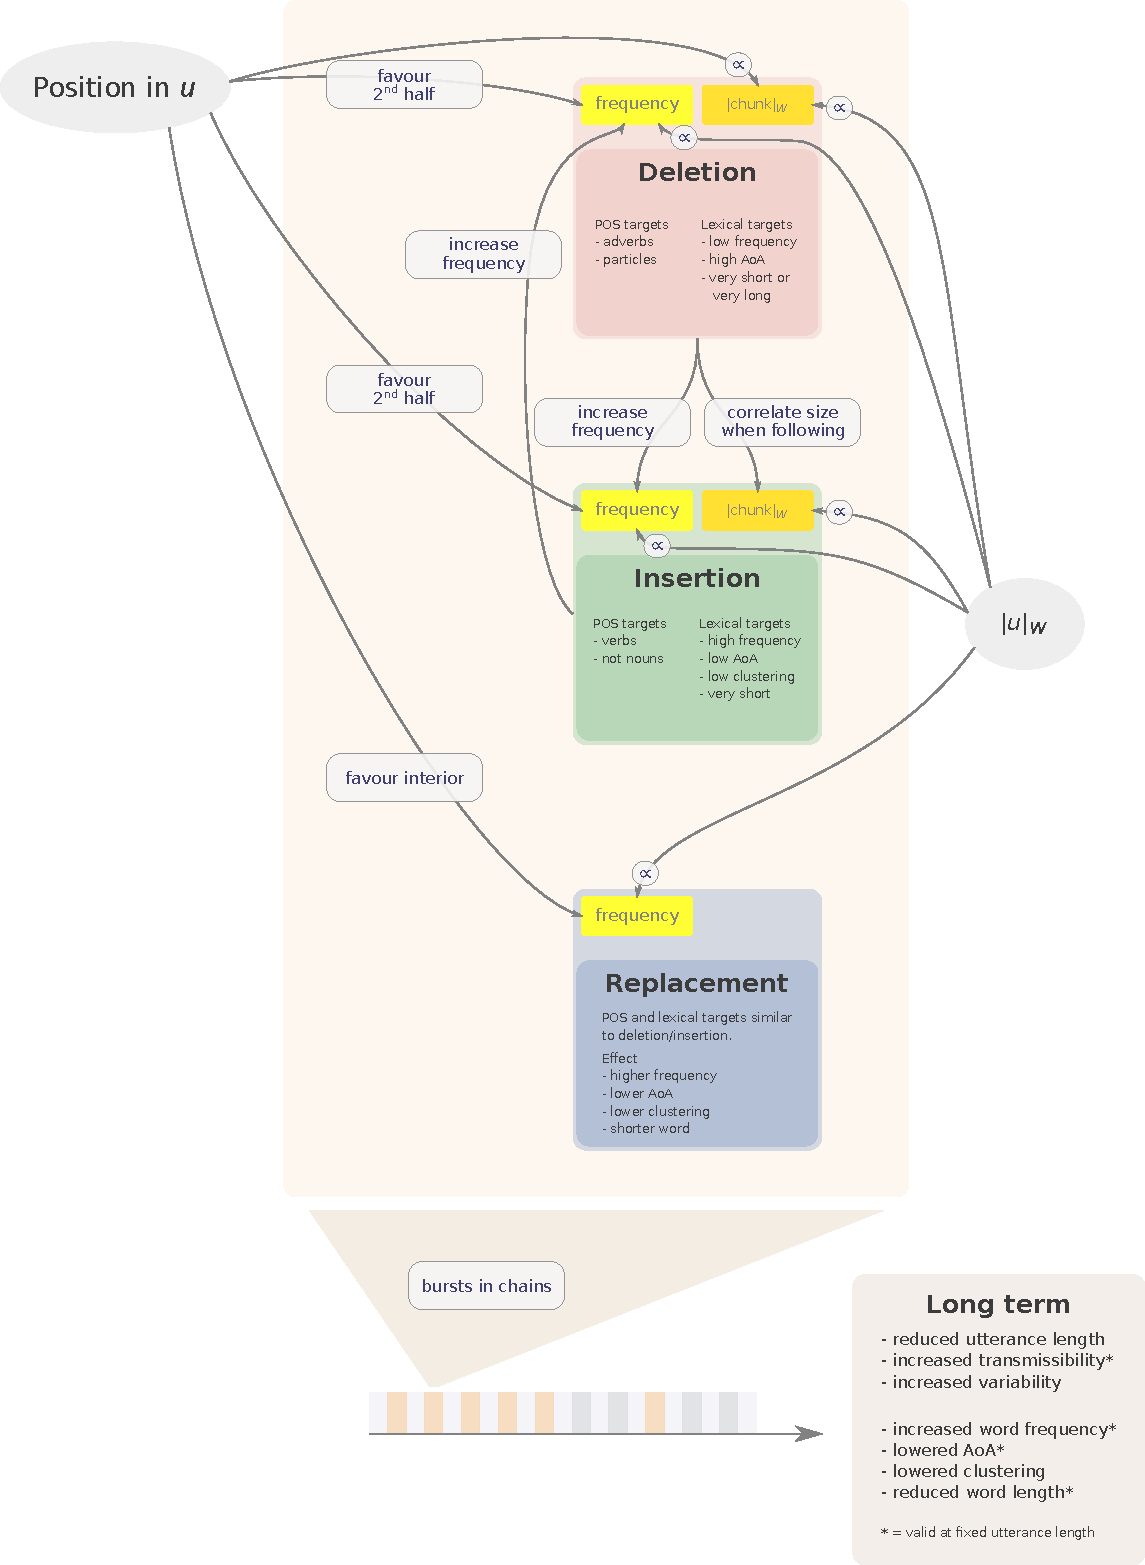
\includegraphics[width=\linewidth]{images/manual/gistr-summary.pdf}
  \caption[Summary of results]{
  \textbf{Summary of results.}
  The upper part of the figure pictures the dependencies observed in the detail of transformations.
  Transformations can be made of deletions, insertions and replacements.
  Deletions and insertions may appear in chunks, but replacements do not.
  Two main factors were shown to influence the likelihood of an operation in a given area of an utterance:
  the position of the words considered for transformation in the utterance, and the overall length of the utterance transformed.
  Arrows thus connect each factor to the frequency and the chunk size of operations, indicating the relationship between the factor and the operation (the $\propto$ symbol indicates that frequency or chunk size is roughly proportional to the factor at the beginning of the arrow).
  Three additional arrows connect deletions and insertions directly, to render the dependencies observed between these two operations.
  A summary of the types of words targeted by each operation is provided inside the darker boxes.
  Finally, the lower part of the figure recalls that transformations appear in bursts in transmission chains, and accumulate to produce the effects summarised in the "Long term" box.
  }
  \label{fig:gistr-summary}
\end{figure}
